\documentclass[12pt]{article}

\usepackage{amssymb,amsmath,amsfonts,eurosym,geometry,ulem,graphicx,caption,color,setspace,sectsty,comment,footmisc,caption,natbib,pdflscape,subfigure,array,hyperref}
\usepackage{xcolor} 
\definecolor{lightblue}{RGB}{100,149,237}
\usepackage{longtable} 
\usepackage{amssymb} 
\usepackage{url}
\usepackage[table,xcdraw]{xcolor}
\usepackage{xcolor}
\usepackage{graphicx}
\usepackage{enumerate}
\usepackage{amsmath}
% \usepackage{amsthm}	
\usepackage{amsfonts, amssymb, float, placeins, tabularx, array, longtable, booktabs, listings} 
\usepackage{natbib}
\usepackage{threeparttable}
\usepackage{graphicx}
\usepackage{subcaption}
\normalem

\onehalfspacing
\newtheorem{theorem}{Theorem}
\newtheorem{corollary}[theorem]{Corollary}
\newtheorem{proposition}{Proposition}
\newenvironment{proof}[1][Proof]{\noindent\textbf{#1.} }{\ \rule{0.5em}{0.5em}}

\newtheorem{hyp}{Hypothesis}
\newtheorem{subhyp}{Hypothesis}[hyp]
\renewcommand{\thesubhyp}{\thehyp\alph{subhyp}}

\newcommand{\red}[1]{{\color{red} #1}}
\newcommand{\blue}[1]{{\color{blue} #1}}

\newcolumntype{L}[1]{>{\raggedright\let\newline\\arraybackslash\hspace{0pt}}m{#1}}
\newcolumntype{C}[1]{>{\centering\let\newline\\arraybackslash\hspace{0pt}}m{#1}}
\newcolumntype{R}[1]{>{\raggedleft\let\newline\\arraybackslash\hspace{0pt}}m{#1}}

\geometry{left=1.0in,right=1.0in,top=1.0in,bottom=1.0in}

\begin{document}

\begin{titlepage}
\title{The Effect of Local Road Maintenance Tax Cuts on House Values
\thanks{Acknowledgements: We are grateful for comments from CK Tang, Guoyang Yang, Dan Boles, Eunjee Kwon, Gary Painter, Olivier Parent, Jeffrey Mills, Nayoung Lee, Matias Cattaneo, and Chris Bollinger, to CoreLogic® for leasing us the housing dataset, to Albert Saiz, Lu Han, Siqi Zheng, David Albouy and other attendees at AREUEA National Conference for their insightful comments. We thank John Schroeder, Public Service Director of Beavercreek township, Ohio, for his insights on funding and maintenance of local roads in Ohio.}}
\author{David Brasington \thanks{Professor, University of Cincinnati} \and Saani Rawat \thanks{PhD Student, University of Cincinnati. Corresponding author: rawatsa@mail.uc.edu}}
\date{\today} 
\maketitle

% \noindent
% \begin{center}
% \textbf{\href{https://drive.google.com/file/d/18fS35u8sh9TMduSvmkO6O6uvLmoLFGa5/view?usp=sharing}{\textcolor{lightblue}{Please click here for the latest draft.}}}
% \end{center}

\begin{abstract}
% \noindent We design a quasi-experiment to study county subdivision-level referendums introduced to renew local road maintenance taxes in U.S., which are typically levied via property taxes. We compare housing sale prices between similar areas that narrowly pass or fail road tax levies and use satellite images to fine-tune an Artificial Intelligence (AI) model for classifying road quality. Our results show that local jurisdictions with close elections that decide to cut road taxes face an average loss of \$163,547 (11\%) in road maintenance funds, experience a 15\% decline in road quality, and suffer a \$15,350 (9\%) drop in housing prices over the course of 10 years relative to similar areas that renew funding. Heterogeneity analysis reveals a stronger decline in urban areas and for expensive houses relative to rural areas and cheaper houses.
\noindent Most studies generally focus on the construction of new transportation infrastructure in developing nations. In this paper, we analyze the maintenance of existing roads in the U.S. which avoids issues of endogeneity coming from the placement of new roads. We design a quasi-experiment to study local referendums introduced to renew road maintenance taxes, which are typically levied via property taxes. We compare housing sale prices between similar areas that narrowly pass or fail road property tax levies and use satellite images to fine-tune an Artificial Intelligence (AI) model for classifying road quality. Our results show that local jurisdictions with close elections that decide to cut road taxes face an average loss of \$163,547 (11\%) in road maintenance funds, experience a 15\% decline in road quality, and suffer a \$15,350 (9\%) drop in house prices over the course of 10 years relative to similar areas that renew funding. Heterogeneity analysis reveals a stronger percentage decline in urban areas and for expensive houses relative to rural areas and cheaper houses.
% Our results show that local jurisdictions with "close elections" which decide to cut local road taxes experience an average loss of \$163,547 (11\%)in road maintenance funds, undergo a 15\% drop in road quality and suffer an average decrease in housing prices of \$15,350 (9\%) over 10 years relative to similar areas that renewed funding.
\\
\vspace{0in}\\
\noindent\textbf{Keywords:} Road Maintenance, Local Taxation, Housing values, Artificial Intelligence \\
\vspace{0in}\\
% \noindent\textbf{JEL Codes:} R42, H71, R10, C21 \\
\noindent\textbf{JEL Codes:} R42, H71, R10 \\

\bigskip
\end{abstract}
\setcounter{page}{0}
\thispagestyle{empty}
\end{titlepage}
\pagebreak \newpage

\doublespacing

% \section*{TAFT Executive Summary}

This paper examines the long-term economic consequences of cutting local road taxes by focusing on a unique quasi-experiment in Ohio. Specifically, it studies communities (cities, villages, and townships) that periodically vote on whether to renew road-maintenance tax levies. When a tax levy renewal narrowly fails, the loss of dedicated road funds provides a natural experiment to measure the causal impact of decreased road spending on housing values.

\noindent {\bf Research Question.} The primary question is: What happens to local house prices when a community votes to cut its road-maintenance tax levy and thus reduces spending on local roads? A secondary question concerns the mechanism driving any observed price changes—namely, whether a drop in funding leads to measurable declines in road quality, which then become capitalized into property values.

\noindent {\bf Data Sources.} Over 3,000 road tax levy referendums from local governments in Ohio (1995–2021). Individual-level house sales data (over 7 million transactions) from CoreLogic®, capturing actual sale prices, demographics, and property characteristics. Satellite imagery for road surface condition, which is analyzed using a fine-tuned Vision Transformer (ViT) model to classify road quality.

\noindent {\bf Identification Strategy.} A regression discontinuity design (RDD) exploits the discrete cutoff at 50\% of the vote. When the levy renewal just fails (vote share against $>$ 50\%), local governments lose a predictable slice of road-maintenance funds. Narrowly passing and narrowly failing areas are assumed to be comparable except for the funding outcome.
Bandwidth selection and local polynomial regression techniques ensure that outcomes are compared within small neighborhoods around the 50\% threshold, strengthening causal inference.

\noindent {\bf Key Findings:} 

\begin{itemize}
    \item {\bf Reduction in Road Quality:} Failed tax renewals result in a significant, visible deterioration in roads. The machine-learning model classifies a 17\% overall decline in road quality in communities that lost their levy.
    \item {\bf Housing Market Impact:} Over a ten-year window, the loss of local road funding leads to approximately a \$15,000 (9\%) decrease in median house prices, starting about four years after the vote. This time lag corresponds to when roads degrade enough for buyers and sellers to notice.
    \item {\bf Heterogeneity:}
    \begin{itemize}
        \item {\bf Urban vs. Rural:} The negative effects on house prices are pronounced in urban areas (about \$25,825 average decline), whereas rural areas display smaller, statistically insignificant price changes.
        \item {\bf Price Quantiles:} Higher-priced homes experience larger devaluations relative to lower-priced homes, suggesting that wealthier households place a greater premium on road aesthetics and quality.
    \end{itemize}
\end{itemize}

\noindent {\bf Mechanisms.} The paper argues for the following mechanisms -

\begin{itemize}
    \item {\bf Funding Shock:} Communities lose a key revenue stream, forcing city officials to postpone road repairs and stretch limited budgets.
    \item {\bf Infrastructure Decay:} Road surfaces gradually degrade, with visible potholes, cracks, and associated driving and commuting costs increasing over time.
    \item {\bf Capitalization into Home Values:} Buyers discount home prices to reflect perceived long-term deterioration of local infrastructure—less curb appeal, higher car repair expenses, and the expectation of future tax shocks or further service cutbacks.
    \item {\bf Short-Run vs. Long-Run Trade-Off:} Residents may initially prefer lower taxes, but the eventual drop in road quality reduces home values. This tension emerges roughly four to five years after a failed levy, highlighting how short-term fiscal relief can yield longer-term property devaluation.
\end{itemize}


\section*{Proposal \& Future Work}

As noted in Executive Summary, in this paper, I demonstrate a causal link between reduced road taxes and a subsequent decline in residential property prices. A key novel component of this project is the use of a fine-tuned Vision Transformer (ViT) model to classify the condition of roads in affected cities. Despite encouraging preliminary results, there are significant methodological, data, and computational hurdles that must be addressed to finalize this research, strengthen its credibility, and extend its policy relevance. The TAFT fellowship will help me address these challenges by providing the necessary resources and support. The tasks I plan to undertake have been explained below.

\begin{itemize}
    \item {\bf Scaling Up the Training Data:} The current ViT model has been fine-tuned on a single, relatively small satellite-imagery dataset. Only a limited subset of images from Ohio were used to validate model performance.
    To improve accuracy and ensure broader applicability, the model needs to be fine-tuned on a larger dataset of Ohio-specific road images. Sourcing and preparing these additional images involve high-resolution captures, systematic geo-referencing, and extensive labeling/annotation work.

    \item {\bf Model Robustness and Multiple ViTs:} Relying on a single ViT architecture could introduce biases or idiosyncrasies in classification. Replicating our results across multiple ViT models with varying hyperparameters or architectures can provide robust checks, confirm generalizability, and address concerns about model dependence.
    Training and validating multiple ViTs is computationally intensive, requiring high-performance computing resources and significant time commitments to manage data pipelines, hyperparameter searches, and model checkpoints.
    
    \item {\bf Uncovering Budget Data from Auditor Reports:} A crucial remaining question is: Exactly how much does road spending decline in each city when a renewal levy fails? To answer this, we must parse Ohio Auditor of State reports and local budget summaries, which are often stored in PDF format and require manual extraction. These data will allow us to measure the precise magnitude and composition of local budget cuts. We will be able to track changes in road-maintenance line items over time (e.g., from year of vote to 3, 5, and 10 years thereafter).
    
    \item {\bf Expanding the Paper with a Dedicated Section on new findings:} A new section focused on road-maintenance budget trajectories will add depth to the empirical analysis. By linking actual spending changes to the observed deterioration in roads, we will provide more direct evidence of the mechanism driving housing-price discounts. This budget-based analysis not only strengthens causal inference but also yields richer policy insights. Cities with a higher proportion of discretionary funds, for example, may compensate for failed levies in ways that mitigate (or exacerbate) road-quality declines.
\end{itemize}

\newpage

\section*{Timeline of Future Work}

\noindent {\bf Months 1–2: Dataset Expansion for Satellite Images}
\begin{itemize}
    \item Acquire (or collect) a larger set of geo-tagged Ohio road images.
    \item Refine and implement labeling/annotation protocols to ensure consistent quality.
\end{itemize}

\noindent {\bf Months 3–5: Model Fine-Tuning and Validation}
\begin{itemize}
    \item Train multiple ViT architectures on the expanded dataset.
    \item Conduct robustness checks across different model configurations.
\end{itemize}

\noindent {\bf Months 6–8: Auditor of State Data Collection}
\begin{itemize}
    \item Systematically download Ohio Auditor of State budget reports for relevant municipalities over the past 20 years.
    \item Develop scripts or rely on manual parsing to extract line-item data on road spending.
\end{itemize}

\noindent {\bf Months 9–10: Integrated Analysis}
\begin{itemize}
    \item Merge newly constructed budget dataset with existing voting, housing, and road-quality data.
    \item Update statistical analyses and include a detailed sub-section on the magnitude and timing of road spending changes following failed levies.
\end{itemize}

\noindent {\bf Months 11–12: Final Write-Up and Policy Extensions}
\begin{itemize}
    \item Produce a full paper draft with consolidated results.
    \item Integrate further policy implications and recommendations based on spending data.
\end{itemize}

\newpage
% \section*{Current Draft}
\begin{center}
    \vspace*{\fill}
    \Huge{{\bf Current Draft}}
    \vspace*{\fill}
\end{center}

\newpage

\section{Introduction} \label{sec:introduction}

Roads are an important form of infrastructure investment that affect firms’ production functions and people’s commuting costs. Many studies examine the importance of roads and how they affect residents' daily lives (\Citeauthor{currier2023} \citeyear{currier2023}; \Citeauthor{adukia2020} \citeyear{adukia2020}; \Citeauthor{asher2020} \citeyear{asher2020}). Some papers emphasize that building new roads increases employment and entry of new firms \citep{gibbons2019new}, thereby increasing economic activity. Other papers point out the potential for worse outcomes in the form of increased inequality between the rich and the poor \citep{hettige2006} and an exodus of workers seeking access to larger labor markets \citep{asher2020}.  
 
In this paper, we highlight the importance of road maintenance by townships, cities and villages (``cities'') in Ohio. We collect data on more than 3,000 elections to renew local road tax levies in Ohio from 1991 to 2021. Using the Dynamic Regression Discontinuity (RD) design, we examine how these exogenous cuts in maintenance spending influence housing prices, focusing on cities where voting results are narrowly decided. Our results reveal that when a city cuts its renewal road taxes, it experiences an 11\% loss in maintenance funds, its road quality declines by 15\% and its house prices decrease by around \$15,350 (9\%), with the effect starting four years after the vote and persisting through several years after the vote. The delayed effect is consistent with the time it takes for roads to deteriorate noticeably. We find that these price effects are driven by urban areas rather than rural areas. We also observe that higher-priced houses experience larger percentage reductions in value than lower-priced houses, indicating a heterogeneous impact across different quantiles. This suggests that higher-income households are more sensitive to road quality than lower-income households. 

% We further find that these price effects are delayed but clear in urban areas, where house prices fall by 7.6\% on average, compared to inconsistent changes in values of houses in rural areas. We also observe that higher-priced homes experience larger reductions in value relative to lower-priced homes, indicating a heterogeneous impact across different quantiles of home prices. This suggests that wealthier households are more sensitive to road quality, as a poor road in front of a high-priced home is more likely to be noticed than a poor road in front of a low-priced home.



% \section{Literature Review} \label{sec:literature}

{\bf Related Literature.} Perhaps the study most related to ours is \cite{asher2020}, which studies the impact of new roads on villages in India. Like our study, its identification strategy is regression discontinuity, although ours is sharp rather than the fuzzy form.  It argues the main obstacle to identification in prior studies is that the placement of new roads is usually correlated with economic (or political) characteristics rather than exogenous. Its findings suggest this is a serious problem with the literature because, unlike prior studies, it finds no strong link between economic growth and new road placement, suggesting that the estimates of previous studies that find a link are driven by road placement in villages that are already growing. \cite{asher2020} touts its use of village-level rather than regional-level data.  We, too, look at economic outcomes at the level of village, city, and township, the most local levels of government.  A surprising finding of \cite{asher2020} is that investment in transportation infrastructure does not affect village incomes, assets, or agricultural output.  Its measure of assets is a village-level average of a series of binary indicators of ownership of a variety of assets, along with separate regressions for the presence of a ‘solid house’, refrigerator, and phone; whereas we study the effect of transportation spending on wages, employment, and housing sale prices.  Of course, our use of a developed geography contrasts with rural villages in India.  Our efforts to achieve identification focus on the maintenance of existing roads, which avoids the endogeneity of the placement of new roads.




We highlight a substantial literature studying the effect of transportation infrastructure on house prices. \cite{hoogendoorn2019house} studies the effect of opening of a tunnel on house prices in the Netherlands, noting that prior research studying transportation infrastructure in developed geographies suffers from reverse causality.  It argues that the opening of the Westerscheldtunnel is a fairly exogenous event, with natural borders that prevent contamination of results by the surrounding environment.  It finds half the capitalized value of the tunnel occurs more than a year before the tunnel opens.  Our data, too, is for a developed nation. \cite{hoogendoorn2019house} argues that the exogeneity of the opening of the tunnel, along with hedonic controls, time trends and postcode fixed effects, identifies its estimates.  One novelty of our study is how ordinary the events are that we study.  While the opening of a new tunnel is important, it is rare.  Votes to renew infrastructure spending are common events in many local governments in the United States, and the quantity of road maintenance spending is regularly chosen by governments around the world, if not by voting then directly by bureaucrats.  It is therefore also important to study the effects of road maintenance spending on house prices. \cite{li2016wheels} studies the overall effect on apartment prices of new subway lines in Beijing, but the estimates may be a net effect of competing factors. \cite{gibbons2005valuing}, studying the construction of new rail stations for the London underground and light rail services, notes that the effect on house prices captures the net effect of better access, increased crime, and increased noise pollution. \cite{levkovich2016effects} looks at the effect of highway development on house prices in the Netherlands.  It separates out accessibility effects from noise pollution and increased traffic effects by looking at different neighborhoods near the highway development.  Its repeat sales difference in differences model finds increased house prices from anticipation effects \citep{kohlhase1991impact}. \cite{beenstock2016hedonic} also finds anticipation effects for house prices (but not new construction) for the development of a highway across Israel. 

We also cite literature assessing the effect of transportation infrastructure on employment and wages. Gibbons et al 2019 analyze how new road infrastructure in Britain affects employment and labor productivity. It finds that while new roads increase area-level employment and the number of firms, they may lead to job reductions in existing firms, coupled with increased wages and output per worker \citep{duranton2012}. This study focuses on the long-term effects of transportation infrastructure on employment, highlighting how improved transit can shift the spatial concentration of industries and workers. Their findings show a significant relationship between transportation improvements and shifts in employment, especially in urban areas. Our results are also consistent with \cite{gibbons2019new} in that changes in road investment do not seem to be related to employment at the establishment level.  Neither \cite{dalenberg1995effects} nor \cite{gibbons2019new} look at the effect of transportation infrastructure in high-poverty areas specifically.  While we find no link between transportation infrastructure investment and wages or employment in our overall sample, we do find a link in high-poverty cities.

{\bf Contribution.} Our paper contributes to the literature on three main fronts. First, we establish a new dataset for our quasi-experiment design, which allows us to study how local tax provision changes impact local infrastructure maintenance and neighborhood home prices. This dataset is unique in that, it contains referendums from local governments in Ohio, which are not typically collectively avaiable anywhere else and linked to local real estate information. This allows us to study the effects of these renewal tax cuts on home sale values at the local level. We also document a novel dataset of road images collected via Google Street Views API for Ohio, through which we are able to classify road quality.

Second, we focus on long-term effects of reduced road taxes funded mainly via property taxes, and observe statistically significant decline in house prices occurring after four years and persisting in later years. This delayed effect highlights how the consequences of road tax cuts are not immediate but gradually accumulate as funding is reduced and roads deteriorate. Our research also identifies heterogeneous impacts, showing that urban areas and higher-priced homes suffer more pronounced price declines. By focusing on distributional effects, the study adds nuance to the understanding of how infrastructure maintenance affects local housing markets.

Third, while much of the literature focuses on infrastructure development and expansion, where the impact of new infrastructure projects is one of the primary concerns and reverse causality is easier to address, we shift the focus to infrastructure maintenance in a developed economy and address endogeneity issues through our quasi-experiment setting. Our approach provides insights that are more relevant for policymakers in advanced economies, where road infrastructure is well established but requires continuous upkeep to avoid economic decline.

{\bf Roadmap.} The rest of the paper is organized as follows. Section \ref{sec:data} provides background information on the data and provides information about the variables used in the study. Section \ref{sec:empirical} outlines the empirical strategy. Section \ref{sec:result} presents the results of the study and shares the relevant robustness checks. Section \ref{sec:conclusion} concludes.

\section{Background \& Data} \label{sec:data}

\subsection{How are roads funded in Ohio?}

Roads in Ohio are funded through a combination of federal, state, and local sources. A significant portion of road funding provided by federal and state governments comes from gas taxes, which are currently set at $\$0.18$ per gallon for federal tax and $\$0.38$ per gallon for Ohio state tax. Additional sources for these 2 levels of government include vehicle registration fees, license plate fees, tolls, and driver's license fees. Funding for local governments largely comes from property taxes. Below, we provide an overview of road funding in Ohio.

{\bf Federal Funding.} U.S Department of Transportation (USDOT) provides funding for road infrastructure through the Federal Highway Administration (FHWA). The FHWA provides funding for the construction, maintenance, and operation of highways, bridges, and tunnels. The federal government provides funding for road infrastructure through the Highway Trust Fund (HTF), which is funded by the federal gas tax. The HTF is divided into two accounts: the Highway Account and the Mass Transit Account. The Highway Account is used to fund highway construction and maintenance, while the Mass Transit Account is used to fund public transportation projects. The federal government also provides funding for road infrastructure through the Surface Transportation Block Grant Program (STBG) or Bipartisan Infrastructure Law \citep{USDOT_BIL_Ohio}, which provides funding for road projects that are not eligible for funding through the HTF. Nevertheless, federal government funding for road infrastructure is generally limited, as in 2022, about 4/5$^\text{th}$ of the funding came from state and local governments \citep{pgpf_htf_explained}.

{\bf State Funding.}
In Ohio, gas taxes, licensing fees and user fees account for $69\%$ of the state's road funding \citep{boesen2021}. The Ohio Department of Transportation (ODOT) is responsible for the allocation of state funds, which are used for both maintenance and new construction. However, about 70\% of funds go to new highway construction, 2\% is given to local governments as grants and only 4\% of state funds is directed towards local road maintenance \citep{odot2023}. The remaining funds are part of payroll \& operating expenses, and other miscellaneous expenses. Hence, most of the road maintenance funding for local, neighborhood-specific roads in Ohio comes from local governments.


{\bf Local Funding.} Local governments in Ohio fund roads mainly through a portion of property taxes, even though there is variation in such funding across the local governments. These municipalities have the authority to levy property taxes specifically for road maintenance, providing a crucial source of funding for the upkeep of local infrastructure. As per our correspondance with the Beavercreek Township, 61\% of their road funds come from property taxes, and only 8\% from gas taxes. Moreover, 77\% of funding for roads in Beavercreek township is provided by the local government and 11\% of overall local government budget is allocated to roadway maintenance \citep{schroeder2025}. Hence, local roads are primarily funded by local governments in Ohio and road maintenance funding is a significant part of the local government's budget.


\subsection{Local Taxation in Ohio}

Ohio consists of 88 counties, each covering about 464 square miles (1,200 square kilometers).  Each county was historically divided into about 15 equally-sized townships, which do not cross county lines.  Citizens can petition to incorporate as a village, which has a different type of government structure than a township and the ability to levy both income and property taxes, whereas townships may only levy property taxes.  When a village exceeds 5,000 population in Ohio it is reclassified as a city.  Villages and cities may cross township and county lines, dissolve, or annex parts of contiguous townships.  Villages, cities and townships, which we call “cities” for brevity, are the most local governmental unit in Ohio. Each local government covers about 18.2 miles$^2$ (47.1 km$^2$) on average. The Ohio Revised Code lets local governments collect a small amount of tax without a vote.  Beyond this limited amount local governments put tax levies on the ballot to ask for additional money from voters.  
The type of tax levy we study is for the renewal of infrastructure spending, which is almost entirely road maintenance.  Levies that pass typically expire, and the most common duration to collect a levy is five years, representing 89\% of the road tax levies in our sample.  If a tax levy is renewed, taxes and funding continue.  If 50\% or fewer votes approve the levy, it fails.  When a tax levy for additional funding fails, there is no increase in funding, but existing funding from other tax levies continues as normal.  When a renewal tax levy fails, funding from that tax levy stops.  99\% of the road tax levies in our sample are property taxes and 1\% are income taxes.

Most regression discontinuity studies that use voting data to look at the impact of funding changes examine new tax levies for additional funding.  \cite{cellini2010value} observes that votes for additional tax money may not be statistically independent; a vote may be proposed until it passes.  We minimize this source of endogeneity of new votes by only considering renewal votes \citep{brasington2017school}.  While a government may choose when to put a vote for additional funding on the ballot and keep proposing the new tax until it is passed, when a vote passes it has an expiration date.  So if a road tax levy for additional funding passes in 2007 to last five years, in 2012 voters will have the chance to renew or reject the tax.  The timing of the vote in 2012 is not endogenous, having been set in 2007.  If voters renew it in 2012, it will be up for renewal again in 2017. 

Road tax levies cover a broad range of activities.  Most of the renewal taxes we consider have stated purposes of “road and bridges repair”, “road repair”, “street fund”, and “street improvements”, although there are less common stated purposes like “repair and maintenance of streets and sewers system” and “resurfacing and rehabilitation of city streets.”  The construction of new roads and bridges, in contrast, would be funded with a tax levy for additional money, not a renewal tax; and it would likely be funded by a bond levy lasting 20 or 30 years.  We eliminate from our dataset stated purposes that might suggest new road construction like a 30-year 1.9-mill new tax in Moscow Village for “permanent improvements” and 0.5-mill new tax for 20 years in Shawnee Hills Village for “general construction and road and bridges repair.” Our dataset includes tax levies like a 2-mill, 5-year renewal in Adams Township (Champaign County) in 1995; a 3-mill, 5-year renewal in Lore City Village in 2016; and a 2.5-mill, 5-year renewal in Pataskala City in 2007.


\subsection{Tax Cuts \& Evidence of Road Quality}

% \subsubsection{Visual Evidence of Road Quality}

\subsubsection{A Tale of Two Cities}

To further understand what differentiates the areas which regularly pass their levies from the areas which often fail to renew their levies, we present two townships in the same county that exhibit very different behavior with respect to successful renewal of their road tax levies. Table \ref{tab:renewals_cuts} provides a comparative analysis of two townships, Andover and Morgan, within Ashtabula County. Despite being in the same county, these townships show contrasting patterns in the renewal of road tax levies. Andover township has consistently passed all its road tax levies, while Morgan township has failed to renew more than half of its levies. This stark difference in voting behavior allows us to examine the impact of road tax levy renewals on road quality within a controlled environment, as both townships share similar geographic,  demographic and economic characteristics.

\begin{table}[ht]
    \centering
    \caption{Andover \& Morgan Townships - Referendum Results}
    \label{tab:renewals_cuts}
    \begin{threeparttable}
    \begin{tabular}{p{4cm}p{3cm}p{3cm}cc}
        \hline
        \multicolumn{5}{l}{\textbf{Panel A. Levy cut Rates}} \\
        County Subdivision  & County & Renewals & Cuts & \% Cut  \\
        \hline
        % Elmore & Village & Ottawa & 20 & 0 \\
        % Bainbridge & Township & Geauga & 19 & 0 \\
        % Ames & Township & Athens & 17 & 0 \\
        % Franklin & Township & Portage & 17 & 0 \\
        Andover & Ashtabula & 16 & 0 & 0\% \\
        Morgan & Ashtabula & 7 & 9 & 44\% \\
        % Auburn & Township & Geauga & 16 & 0 \\
        % Chester & Township & Geauga & 16 & 0 \\
        % Waterloo & Township & Athens & 15 & 1 \\
        % Hiram & Township & Portage & 15 & 0 \\
        % Ashtabula & Township & Ashtabula & 14 & 0 \\
        \\
        \hline
        \multicolumn{5}{l}{\textbf{Panel B. Township Characteristics}} \\
        Covariates & Andover & Morgan & Renewals & Cuts \\
        \hline
        Morgan & Township & Ashtabula & 7 & 9 \\
        Rush & Township & Champaign & 11 & 9 \\
        Wayne & Township & Champaign & 5 & 8 \\
        Rose & Township & Carroll & 6 & 6 \\
        Perry & Township & Morrow & 4 & 6 \\
        Washington & Township & Scioto & 10 & 6 \\
        Waynesville & Village & Warren & 2 & 6 \\
        Trumbull & Township & Ashtabula & 3 & 5 \\
        Thompson & Township & Geauga & 7 & 5 \\
        Paint & Township & Holmes & 8 & 5 \\
        \hline
    \end{tabular}
    \begin{tablenotes}
        \small
        \item This table shows the ten cities in Ohio with the largest number of renewed road maintenance levies (Panel A) and the most levies that failed to renew funding (Panel B). The table also provides subdivision type and county for each city. Townships belonging to Ashtabula county have been highlighted.  
    \end{tablenotes}
    \end{threeparttable}
\end{table}

% \begin{figure}[htbp]
%     \centering
%     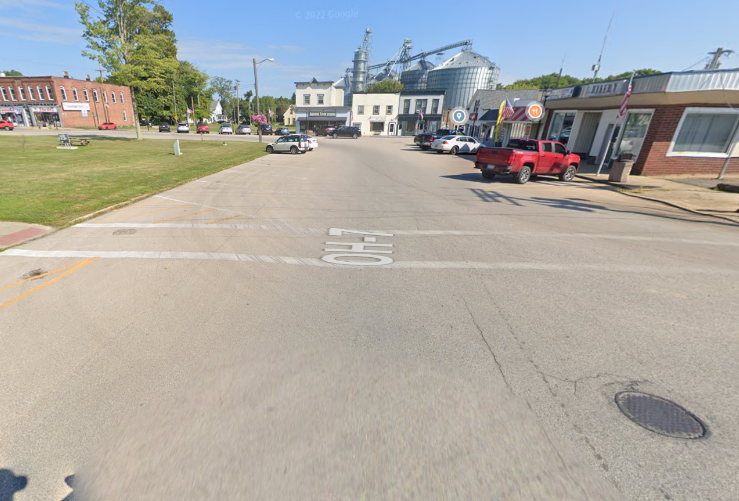
\includegraphics[width=\textwidth,keepaspectratio]{images/andover_township_14grandarmy_2022.png}
% \end{figure}

\begin{figure}[htbp]
    \centering
    \begin{minipage}{0.49\textwidth}
        \centering
        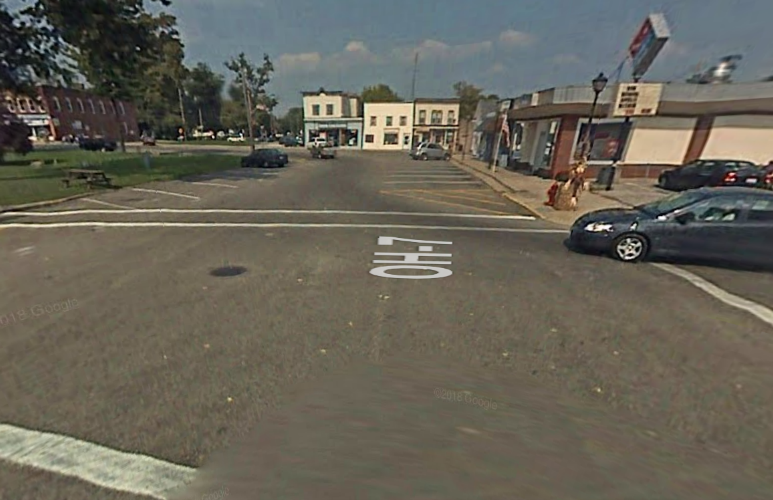
\includegraphics[width=\textwidth,keepaspectratio]{images/andover_township_14grandarmy_2007.png}
        \caption*{Grand Army of the Republic Hwy: 2007} % * suppresses numbering
        \label{fig:andover_2007}
    \end{minipage}
    \hfill
    \begin{minipage}{0.49\textwidth}
        \centering
        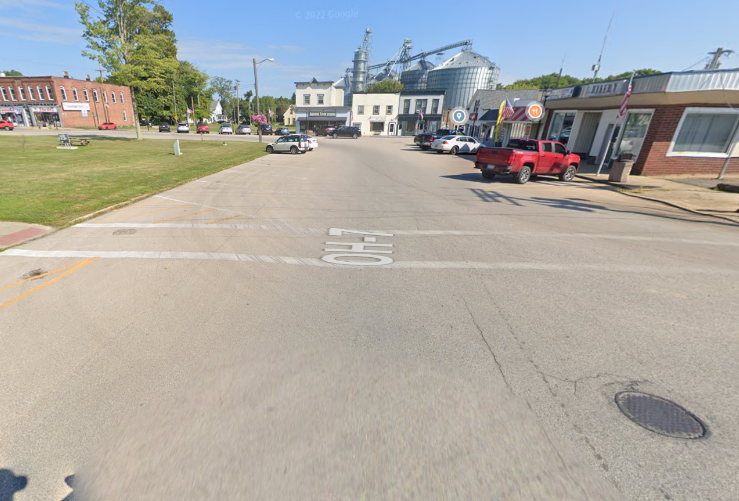
\includegraphics[width=\textwidth,keepaspectratio]{images/andover_township_14grandarmy_2022.png}
        \caption*{Grand Army of the Republic Hwy: 2022}
        \label{fig:andover_2022}
    \end{minipage}
    \caption{Andover township - Road quality}
    \label{fig:rd_andover}
\end{figure}

\begin{figure}[htbp]
    \centering
    \begin{minipage}{0.49\textwidth}
        \centering
        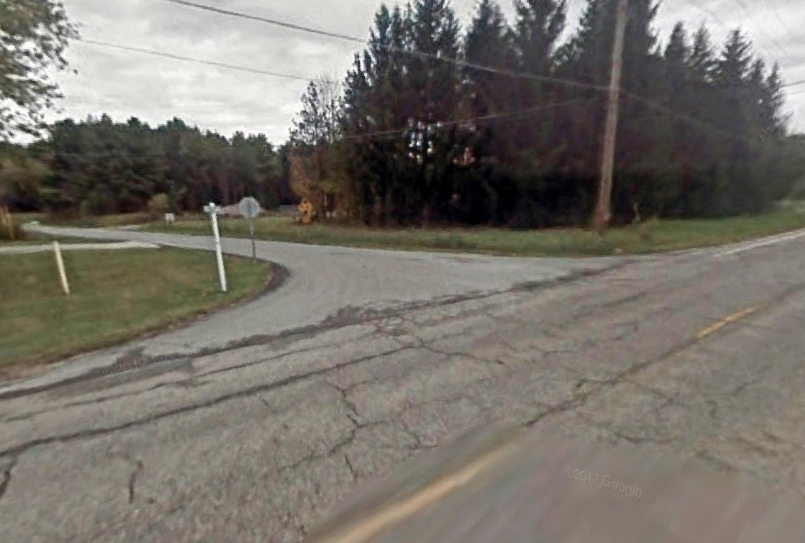
\includegraphics[width=\textwidth,keepaspectratio]{images/morgan_township_2801OH-45_2009.png}
        \caption*{OH-45: 2009}
        \label{fig:morgan_oh_2009}
    \end{minipage}
    \hfill
    \begin{minipage}{0.49\textwidth}
        \centering
        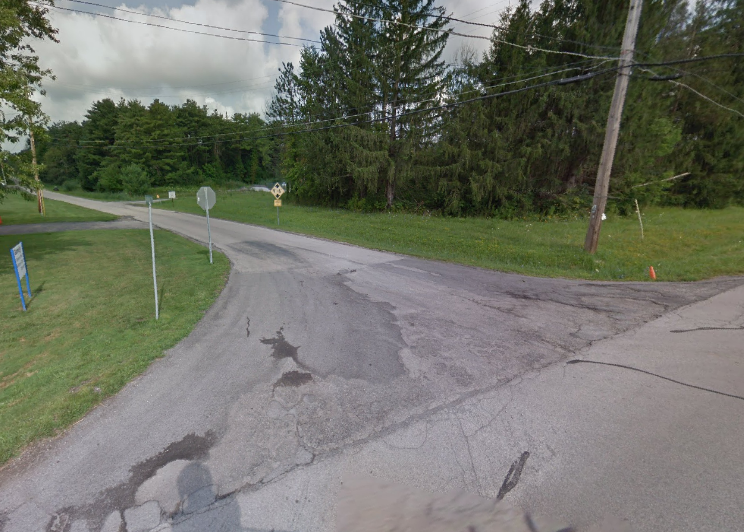
\includegraphics[width=\textwidth,keepaspectratio]{images/morgan_township_2801OH-45_2018.png}
        \caption*{OH-45: 2018}
        \label{fig:morgan_oh_2018}
    \end{minipage}
    \caption{Morgan township - Road quality}
    \label{fig:rd_morgan}
\end{figure}


Table \ref{tab:max_renewals_cuts} shows that there are certain cities which always renew their road tax levies and other cities which often cut their renewal tax levies. Interestingly, we find two townships, Andover and Morgan, which belong to the same county of Ashtabula but exhibit very different behavior in terms of their voting patterns. Andover township passed all the road tax levies that were up for election whereas Morgan township failed to renew more than 56\% of its renewal levies. Since both the townships belong to the same county and have similar characteristics, we can effectively identify whether cutting road spending via road tax levies have a tangible impact on the quality of roads in the area. For this, we leverage Google Street Maps (GSM). Since photos of roads on GSM are time-stamped and the same area can have photos from different points in time, this feature allows us to observe the evolving condition of roads in these neighborhoods over time. For instance, we can observe the major streets of Andover township and compare them with the main streets of Morgan township. We checked whether there were any road tax renewals that took place between these available dates and then observed whether the road conditions improved, stayed the same or deteriorated during this period. Figure \ref{fig:rd_andover} shows Grand Army of the Republic Hwy, a specific hub in Andover, for periods 2007 and 2022. The road quality appears to have been maintained well over the years, indicating that consistent renewal of road tax levies contributes to sustained road infrastructure quality. In contrast, Figure \ref{fig:rd_morgan} illustrates the condition of OH-45 and W Water St in Morgan township for the years 2009 and 2018. The deterioration as well as continuation of poor road quality is evident, suggesting that the failure to renew road tax levies has a tangible negative impact on roads. The disparity in road conditions between Andover and Morgan townships may be suggestive of the broader economic implications of fiscal policy decisions at the local level, particularly how underinvestment in infrastructure can lead to tangible declines in public asset quality and potentially hinder economic growth and development.

\subsubsection{Assessing Road Quality using Satellite Imagery} \label{sec:road_quality}

To understand the effect of cutting local road tax on road quality, we fine-tune a Vision Transformer (ViT) model, gpt-4o by OpenAI, on satellite imagery data from \cite{brewer2021}. Following the seminal work on text-based Transformers in Natural Language Processing (NLP) by \cite{vaswani2017attention}, ViTs were introduced by Google Brain's team and are part of a recent class of deep learning models that have shown to outperform Convolutional Neural Networks (CNNs) on image classification tasks \citep{dosovitskiy2020image}. Below, we outline the steps we take to assess road quality using the ViT model.


% We use the ViT model to classify road images into three categories: good, average, and poor. We then use the classification results to assess the quality of roads in different neighborhoods in Ohio. We collect road images for areas that were within the average effective RD bandwidth provided in Table \ref{tab:median_sale_amount} and ensure that we have pre and post referendum images for both, the treatment and control groups. This allows us to construct a novel database of road images and assess the impact of cutting local road tax on road quality.

{\bf Satellite Images for fine-tuning.} In order to enable ViTs to accurately predict road quality, we needed large-scale road-image data to fine-tune OpenAI's gpt-4o, a Large Language Model (LLM) with multi-modal ability that has shown to outperform various other models and benchmarks \citep{achiam2023gpt}. We use the road-image dataset by \cite{brewer2021} which consists of 53,677 labeled images of road infrastructure for U.S. from 1,000 cities across the United States. The dataset includes images of roads in different conditions, and a classification representing quality of the road: 0 (poor), 1 (decent) and 2 (high). 

{\bf Ohio Satellite Images.} We use satellite images from Google Earth Pro for roads in different neighborhoods in Ohio. We collect road images for areas that were within the average effective RD bandwidth provided in Table \ref{tab:median_sale_amount} and ensure that we have pre and post referendum images for both, the treatment and control groups. This allows us to construct a novel database of road images, which we use to classify road quality for areas that were part of our quasi-experiment. 


{\bf Fine-tuning process.} Fine-tuning a ViT involves taking a pretrained model and adapting it for specific image-classification task. We fine-tune gpt-4o, a pretrained model with over 200 billion parameters, on the road-image dataset by \cite{brewer2021} to classify road images into three categories: 0, 1 and 2. Next, we divide the data into traning and validation datasets. Using OpenAI's API, we set up a training seed, convert the images into their corresponding base64 encoding and fine-tune the model on the road-image dataset for 10 epochs with a batch size of 9 and a learning rate multiplier of 2. For further details on fine-tuning and results, see Appendix \ref{sec:appxc1}. 

% We use the classification results to assess the quality of roads in different neighborhoods in Ohio. We collect road images for areas that were within the average effective RD bandwidth provided in Table \ref{tab:median_sale_amount} and ensure that we have pre and post referendum images for both, the treatment and control groups. This allows us to construct a novel database of road images and assess the impact of cutting local road tax on road quality.

% {\bf Predicting Road Quality.} 




% \bf{Analyzing satellite images.} Following \cite{brewer2021}

% \bf{Street Images.} We utilize a 

% \clearpage

\subsection{Road Maintenance Funding}



\subsection{Running Variable}

The running variable plays a critical role in regression discontinuity.  In our case it represents the proportion of votes against the renewal of a road tax levy.  A vote share of less than 50 means the tax will no longer be collected, and road funding from that particular tax levy will stop.  Other road tax levies may continue to be in effect, and funds from current expense tax levies may still be used for road maintenance.  There are 3,188 votes in our sample, 83\% of which renew the tax, and 17\% of which cut taxes and road maintenance.

We quantify the size of the cut in road spending a city faces in two ways.  First, not every city has a tax levy in effect specifically for roads, but every city has current expense tax funding.  Our mean 1.9 mill road tax represents 13.6\% of current expense funding, indicating that cities that fail to renew a road tax levy face a moderate reduction in funding.  We also investigate the drop in road expenditures by sampling financial audits of cities in our sample whose renewal tax levies fail, finding an average drop of \$218,808 in road spending one year later.  This \$218,808 drop represents a 34\% decrease in road spending.  
In our sample, the mean vote share against the tax levy is 0.38, which is essentially the same as the median of 0.36.  The standard deviation is 0.15, so that the typical levy that fails represents a little less than one standard deviation away from the mean. The Great Financial Crisis falls in the middle of our dataset, so readers might wonder if voting behavior was affected, but we find vote share the same to two decimal points during and outside the years 2008-2009. 


\subsection{Outcome Variables}


{\bf Median Housing Prices.} Our house price data comes from a CoreLogic® dataset of actual sales transaction prices in Ohio from 1995 through 2021 containing over 7 million observations. The dependent variable, \textit{Median House Price}, reflects the median sale price of houses within a specific city and year. For example, for the houses sold in Delaware Township during the year 2002, the median sale price was \$205,041. We take precaution to only include arm’s-length transactions, and we restrict our attention to single-family residential structures for comparability.  The overall sample mean for the 10-year period from the time of vote considered in this study is \$166,082 in constant 2010 dollars with a standard deviation of \$372,135 which suggests presence of some outliers. Although our use of median sale price addresses outliers, one of our robustness checks drops 1\% tails and re-estimates the treatment effects.  The mean for this winsorized sample is \$150,375 in constant 2010 dollars with a standard deviation of \$116,020. 

\begin{figure}[ht]
    \centering
    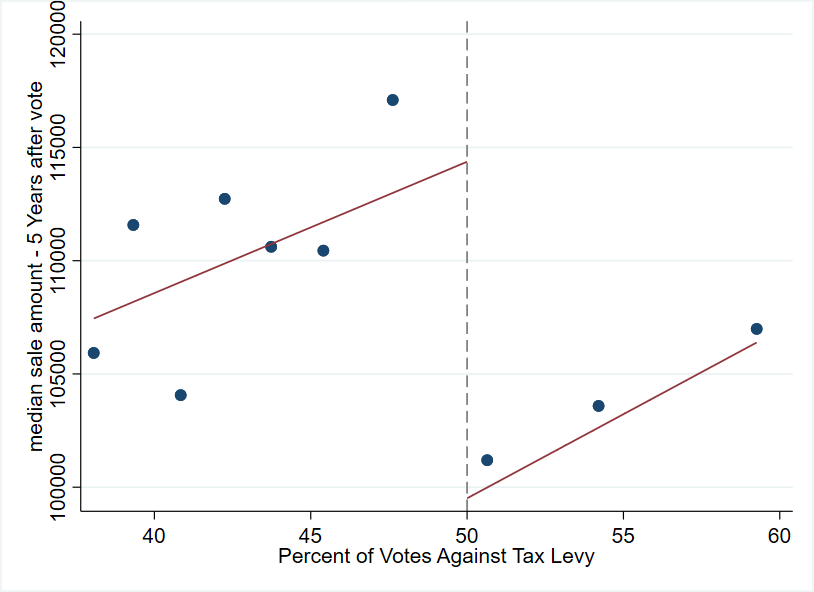
\includegraphics[width=0.8\textwidth,keepaspectratio]{images/rd_plot_year_5_after_vote.png}
    \caption{Median Sale Price of Homes: 5 years after vote}
    \label{fig:hp_year5_after}
\end{figure}

Figure \ref{fig:hp_year5_after} shows house prices from 5 years after the vote graphed against the percent of votes for the tax levy. The points represent the mean house price for the 10 representative bins of vote shares for the average effective bandwidth around the cutoff of 50\%. The graph shows a clear discontinuity in house prices at the cutoff, which is the basis for our identification strategy. We observe a sharp decline after the cutoff in house prices, indicating that the failure to renew a road tax levy has a negative impact on house prices.


\subsection{Covariates}

Covariates can be useful in regression discontinuity studies, although they are not necessary for the identification of treatment effects.  One use of covariates is to increase the precision of treatment effect estimates.  The other is to see if cities that barely pass and fail tax levies are similar to each other like the theory of regression discontinuity says they should be. Table \ref{tab:variable_means_sd} shows covariate means for both the global sample of all votes in the data set as well as the local sample within a representative effective bandwidth of the 0.50 cutoff. The effective bandwidth displayed in Table \ref{tab:variable_means_sd} is the mean bandwidth for all the housing outcome regressions. The first columns for the global sample show similar values of characteristics between cities that renew and cut road taxes and spending, but it is the two rightmost columns that are critical for the credibility of the regression discontinuity design.   

Table \ref{tab:variable_means_sd} demonstrates the covariate balance between cities that renew their tax levies and those that do not, indicating similar demographic and economic profiles across both groups. The data, captured at the time of the vote, shows minimal differences within the effective bandwidth: the mean population differs by only 224 from a base of 5,220, and median family income varies by \$190 from a base of \$60,269, measured in 2010 U.S. dollars. Other variables, including poverty rates, single-parent household percentages, educational attainment, age distribution, and racial composition, show differences of less than one percentage point, reinforcing the comparability of the two groups.


\begin{longtable}{p{4cm}cccccc}
    \caption{Variable Means \& Standard Deviation by Tax Levy Renewal Status} \label{tab:variable_means_sd} \\
    \hline
    Variable & \multicolumn{3}{c}{Global} & \multicolumn{2}{c}{Effective} \\
    \cmidrule(lr){2-4} \cmidrule(lr){5-6}
    & Full Sample & Renewed & Cut & Renewed (Control) & Cut (Treatment) \\
    \hline
    \endfirsthead

    \multicolumn{6}{c}{{\bfseries \tablename\ \thetable{} -- continued from previous page}} \\
    \hline
    Variable & \multicolumn{3}{c}{Global} & \multicolumn{2}{c}{Effective} \\
    \cmidrule(lr){2-4} \cmidrule(lr){5-6}
    & Full Sample & Renewed & Cut & Renewed (Control) & Cut (Treatment) \\
    \hline
    \endhead

    \hline \multicolumn{6}{r}{{Continued on next page}} \\
    \endfoot

    \hline
    \endlastfoot

    \multicolumn{6}{l}{\textbf{Panel A. Covariates}} \\
    Population & 5,074 & 5,134 & 4,769 & 5,220 & 4,996 \\
               & (7,942) & (8,030) & (7,478) & (8,205) & (7,420) \\
    Poverty Rate & 0.11 & 0.11 & 0.11 & 0.11 & 0.10 \\
                 & (0.08) & (0.08) & (0.07) & (0.08) & (0.07) \\
    \% with Kids & 0.39 & 0.39 & 0.40 & 0.39 & 0.39 \\
                 & (0.08) & (0.08) & (0.08) & (0.08) & (0.07) \\
    \% Households with Children under 18 & 0.09 & 0.09 & 0.09 & 0.09 & 0.08 \\
                                         & (0.06) & (0.06) & (0.05) & (0.06) & (0.05) \\
    \% Less than High School Education & 0.16 & 0.15 & 0.18 & 0.17 & 0.18 \\
                                       & (0.11) & (0.11) & (0.10) & (0.11) & (0.09) \\
    \% Some College Education & 0.25 & 0.25 & 0.24 & 0.25 & 0.24 \\
                              & (0.06) & (0.06) & (0.06) & (0.06) & (0.07) \\
    \% Unemployment Rate & 0.05 & 0.05 & 0.05 & 0.06 & 0.05 \\
                         & (0.04) & (0.04) & (0.03) & (0.04) & (0.03) \\
    \% Renters & 0.20 & 0.20 & 0.20 & 0.20 & 0.19 \\
               & (0.11) & (0.11) & (0.10) & (0.11) & (0.09) \\
    \% White & 0.96 & 0.96 & 0.97 & 0.97 & 0.96 \\
             & (0.07) & (0.08) & (0.07) & (0.08) & (0.08) \\
    \% Black & 0.02 & 0.02 & 0.02 & 0.02 & 0.02 \\
             & (0.07) & (0.07) & (0.06) & (0.07) & (0.07) \\
    \% Married & 0.59 & 0.59 & 0.60 & 0.60 & 0.61 \\
               & (0.09) & (0.09) & (0.08) & (0.09) & (0.08) \\
    \% Separated & 0.01 & 0.01 & 0.01 & 0.01 & 0.01 \\
                 & (0.01) & (0.01) & (0.01) & (0.01) & (0.01) \\
    Income Heterogeneity Index & 0.10 & 0.10 & 0.09 & 0.09 & 0.09 \\
                               & (0.08) & (0.08) & (0.07) & (0.07) & (0.06) \\
    Median Family Income & 61,014 & 61,445 & 58,837 & 60,269 & 60,079 \\
                         & (17,694) & (18,283) & (14,177) & (15,687) & (14,143) \\
    \% Under 5 Years Old & 0.06 & 0.06 & 0.06 & 0.06 & 0.06 \\
                         & (0.02) & (0.02) & (0.02) & (0.02) & (0.02) \\
    \% Aged 5 to 17 & 0.20 & 0.20 & 0.21 & 0.20 & 0.20 \\
                    & (0.05) & (0.05) & (0.04) & (0.05) & (0.04) \\
    \% Aged 18 to 64 & 0.60 & 0.60 & 0.60 & 0.60 & 0.60 \\
                     & (0.05) & (0.05) & (0.05) & (0.05) & (0.04) \\
    \% Racial Minority & 0.04 & 0.04 & 0.03 & 0.03 & 0.04 \\
                       & (0.07) & (0.08) & (0.07) & (0.08) & (0.08) \\
    Number of Observations & 3,188 & 2,661 & 527 & 694 & 273 \\
    \\
    \multicolumn{6}{l}{\textbf{Panel B. Outcome Variables}} \\
    \textit{a) Median House Price} & & & & & \\
    t - 3 & 106,067 & 107,502 & 102,766 & 106,771 & 104,201 \\
          & (52,988) & (60,197) & (50,794) & (53,461) & (51,794) \\
    t - 2 & 105,528 & 107,211 & 101,456 & 106,207 & 103,713 \\
          & (53,242) & (60,893) & (48,438) & (54,162) & (50,786) \\
    t - 1 & 107,706 & 108,234 & 104,575 & 108,401 & 105,843 \\
          & (53,544) & (62,437) & (51,343) & (54,665) & (50,491) \\
    \textit{b) Median House Price (\%)} & & & & & \\
    t - 3 & 1,504 & 1,752 & 1,728 & 1,446 & 1,695 \\
          & (3,848) & (4,006) & (3,642) & (3,887) & (3,739) \\
    t - 2 & 1,429 & 1,734 & 1,680 & 1,388 & 1,562 \\
          & (3,693) & (3,978) & (3,612) & (3,769) & (3,462) \\
    t - 1 & 1,387 & 1,724 & 1,668 & 1,341 & 1,538 \\
          & (3,628) & (3,993) & (3,598) & (3,683) & (3,460) \\
    \textit{c) Median House Price per square foot} & & & & & \\
    t - 3 & 31,764 & 31,892 & 32,531 & 32,367 & 32,401 \\
          & (8,868) & (8,428) & (10,090) & (9,657) & (8,898) \\
    t - 2 & 31,714 & 32,083 & 32,048 & 31,571 & 32,166 \\
          & (8,630) & (8,392) & (9,224) & (8,723) & (8,372) \\
    t - 1 & 31,764 & 32,399 & 32,399 & 31,579 & 32,367 \\
          & (8,868) & (9,716) & (9,716) & (8,623) & (9,657) \\
\end{longtable}

% \begin{tablenotes}
%     \small
%     \item Notes: Panel A shows covariates used in estimating the treatment effect of failing to renew a road tax levy. Covariate means at the time of the vote are shown along with standard deviations in parentheses. The unit of observation is city-year. 'Income' is median family income in constant 2010 U.S. dollars. 'Global' refers to the full sample of city-year votes; 'Effective' refers to city-year votes within the mean estimated optimal bandwidth of 10 percentage points around the cutoff for years 1995 through 2021. The treatment group reflects cutting road funding by failing to renew the road tax levy. The control group reflects maintaining road funding by renewing the road tax levy. Panel B shows means of outcome variables for placebo years t - 3, t - 2, and t - 1.
% \end{tablenotes}


Table \ref{tab:variable_means_sd} shows that the treatment and control groups are well-balanced with respect to the covariates considered, suggesting that the groups are comparable and any observed differences in outcomes can more confidently be attributed to the treatment effect rather than to pre-existing differences.

\subsection{Testing how well the data meets the assumptions of RDD}
The assumptions of regression discontinuity are minimal compared to other identification strategies. One is that no agent, while having some influence, may precisely assign observations to a specific value of the running variable. In our context, it means that the election results are not determined prior to when the ballot takes place. In other words, no individuals, organizations, higher levels of government, foreign governments, or the firm that programs the voting machines are dictating the precise vote share for the renewal road tax levy referendums raised by a city. The standard way to test this assumption is to perform a density test like that of \cite{cattaneo2020simple}, which is based on the idea that manipulation of elections might cause a clustering of votes just to one side of the cutoff, with a pronounced drop-off on the other side of the cutoff. The $p$-value of this density test is 0.98. A histogram of vote share is shown in Figure \ref{fig:running_var_hist} that graphically illustrates the lack of abrupt change in density.

\begin{figure}[ht]
    \centering
    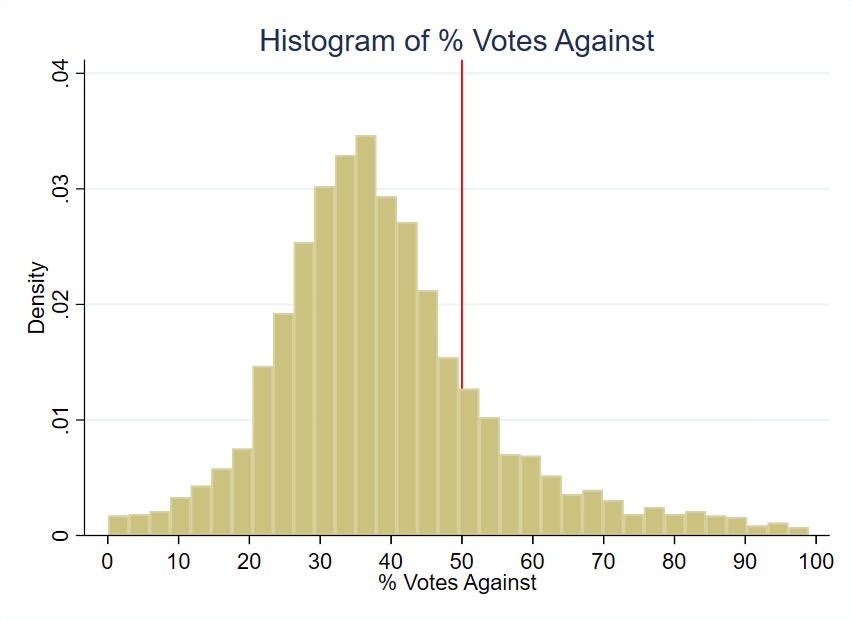
\includegraphics[width=\textwidth,keepaspectratio]{images/votes_pct_against_histogram.png}
    \caption{Histogram of Running Variable}
    \label{fig:running_var_hist}
\end{figure}

Although Table \ref{tab:variable_means_sd} shows covariate balance between sets of cities that pass and fail to renew road tax levies, covariate values could still jump from one side of the cutoff to another. A drop in education levels, for example, could cause a drop in house prices that might coincide with a change in treatment, so that what might look like a treatment effect from cutting taxes and spending might in fact be caused by lower education levels.  Graphs of covariate smoothness around the cutoff are found in the Appendix \ref{sec:appxb}. A formal way to assess covariate smoothness is to use each covariate as an outcome variable in a regression of the running variable and a treatment effect dummy. When we do so, the $p$-value of the treatment effect dummy varies from 0.13 to 0.98, indicating no statistically significant jump in covariate values. 


\section{Empirical Strategy} \label{sec:empirical}

We follow a model of sharp Regression Discontinuity Design (RDD), as detailed in \cite{calonico2019regression}. A formal description of the model is provided below. Let $Y_{it}$ represent the outcome variable for city, village or township $i$ at year $t$. The outcome variables we study include house prices, wages, and employment. Drawing from the Rubin causal model, we use potential outcomes notation to describe $Y_{it}(1)$ as a potential outcome variable if exposed to treatment and $Y_{it}(0)$ as the potential outcome variable in absence of treatment i.e. our control. We define treatment as failure of a city, village or township to renew its road maintenance tax levy. Let $T_{it} \in \{0,1\}$ represent cities that receive treatment (1) or not (0) based on voting at year $t$, so that our realized outcome is represented by the following equation:

$$
Y_{it} = Y_{it}(1) \times T_{it} + Y_{it}(0) \times (1-T_{it})
$$

Let $X_{it}$ be the running variable that determines whether a realized outcome variable was treated or not based on some cutoff $\underbar{x}$. In our study, the running variable is the percent of votes against the renewal tax levy and the cutoff is 50 percent. Let $Z_{it}$ be our vector of covariates and $\tau$ be our parameter of interest i.e. the treatment effect. This parameter of interest measures the causal effect of cutting road maintenance spending on different outcome variables. Under the assumption of continuity at the cutoff $\underbar{x}$, the RDD allows us to compute the average treatment effect $\tau = \mathbb{E}(Y_{it}(1) - Y_{it}(0) | X_{it} = \underbar{x})$. We employ both local polynomial and local randomization approaches to compute the estimate for $\tau$, which we call $\hat{\tau}$.

To observe the persistence of treatment effects, we develop an event study-styled estimator that tracks the outcome variable for different values in future. The regression equation takes the form -

$$
Y_{i(t+r)} = \alpha_r + T_{i(t+r)} \tau_r + X_{i(t+r)} \beta_r + T_{i(t+r)} X_{i(t+r)} \theta_r + Z_{i(t+r)} \gamma_r + \epsilon_{i(t+r)}
$$

\noindent where $r \in \{-3,-2, ..., 10 \}$, $\alpha_r$ is the intercept, $\beta_r$ is the coefficient on the running variable $X_{i(t+r)}$, $\theta_r$ is the coefficient of the interaction term, $\gamma_r$ is a vector of coefficients for covariates matrix $Z_{i(t+r)}$ and $\epsilon_{i(t+r)}$ is the idiosyncratic error term. Our parameter of interest, $\tau_r$ measures the causal effect of cutting road maintenance spending on different outcome variables for different values of $r$. We estimate the treatment effect for different values of $r$ to observe the persistence of treatment effects and consider the possibly of placebo effects. 

The above equation has been described in detail in \cite{calonico2019regression} and is called the covariate-adjusted RDD estimator. We use the bandwidth selection method described in \cite{calonico2019regression} to choose a bandwidth $h$ and then conduct a local linear polynomial regression after choosing a weighting scheme. The bandwidth $h$ determines size of the neighborhood around the cutoff $\underbar{x}$, where the neighborhood is $(\underbar{x}-h, \underbar{x}+h)$. Only observations with values of the running variable within this neighborhood are used to compute the treatment effect estimate $\hat{\tau}$ and, for a small enough neighborhood, the continuity assumption central to the RDD estimator is satisfied. The weighting scheme $k$ determines the weights of the observations within the neighborhood $(\underbar{x}-h, \underbar{x}+h)$ and is another important factor in determining $\hat{\tau}$. The most common types of weighting schemes are uniform, triangular and Epanechnikov. We use the default Mean Squared Error Regression Discontinuity (MSERD) method to compute the effective bandwidth ($h$) and bias bandwidth ($b$) for each outcome variable. This method identifies the bandwidth that minimizes the trade-off between bias and variance of the treatment effect estimate. All observations are used to estimate $h$ and $b$, but only the observations within the selected bandwidth $h$ i.e. effective observations within $h$ percentage points on either side of the 0.50 vote share cutoff are used to identify our treatment effect estimates.



\section{Results} \label{sec:result}

% First, we share the results for house prices. Next, we present the results for employment and wages outcome variables.

% \subsection{Local government spending}



\subsection{Road Quality decline} \label{sec:road_quality_decline}

 To assess the impact of cutting local road taxes on road quality, we utilized a fine-tuned Vision Transformer (ViT) model, leveraging labeled satellite imagery data for U.S. roads. The ViT model, fine-tuned using a large dataset of road images, assigned quality ratings on a scale of 0 (poor) to 2 (high) to our collected satellite imagery for Ohio neighborhoods, as explained in Section \ref{sec:road_quality}. We compared road quality ratings from the fine-tuned ViT model before and after the referendum in areas that failed to renew their road tax levy versus those that successfully passed the levy. These results are summarized in Table \ref{tab:roadquality_estimates}. 

% \begin{figure}[htbp]
%     \centering
%     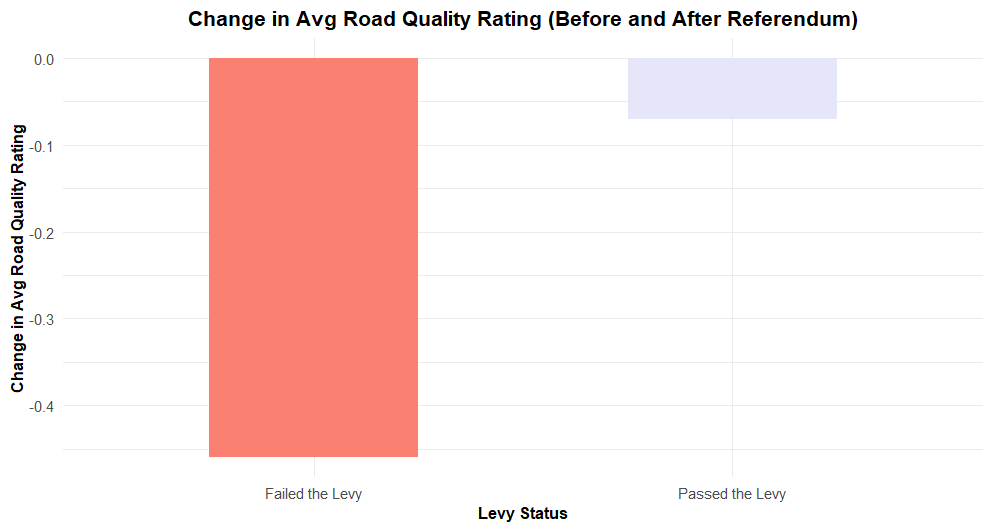
\includegraphics[width=\textwidth,keepaspectratio]{images/road_quality_change.png}
%     \caption{Change in Road Quality Ratings Before and After Referendum}
%     \label{fig:road_quality_change}
% \end{figure}

\begin{table}[ht]
    \centering
    \caption{Effect of Referendum Outcome on Road Quality}
    \label{tab:roadquality_estimates}
    \begin{threeparttable}
    \begin{tabular}{lcc}
    \hline\hline
     & \textbf{Cut Levies} & \textbf{Maintained Levies} \\
    \hline
    \\[-0.3cm] % Adds space before the row to properly display significance stars
    Change in Road Quality after a Referendum 
     & -0.444\textsuperscript{**} & 0.067 \\[0.2cm] % Adds space after the first row
     & (0.210) & (0.340) \\  
    \hline
    \end{tabular}
    \begin{tablenotes}
    \small
    \item \textit{Notes:} Each column represents a separate regression of the predicted  road-quality classification variable on an indicator for the post-election period for areas with close elections, as determined by the effective bandwidth around the RD cutoff. “Cut Levies” refers to jurisdictions that failed to renew their road tax levies, while “Maintained Levies” refers to jurisdictions that renewed. Standard errors are shown in parentheses. 
    
    \item Significance levels: 
    \textsuperscript{*}p $<$ 0.10,  
    \textsuperscript{**}p $<$ 0.05, 
    \textsuperscript{***}p $<$ 0.01.
    \end{tablenotes}
    \end{threeparttable}
\end{table}


Areas that cut their renewal road tax levies experienced an average decline in road quality ratings of -0.444 points, equivalent to a 15\% deterioration in road quality relative to the three-point scale.\footnote{Calculated as -0.444/3 = 15\%.} In contrast, areas that maintained their tax levies experience did not experience a statistically significant change, suggesting effectively no deterioration in road quality. In neighborhoods where renewal taxes were cut, the decline in road quality highlights the potential long-term implications of fiscal policy decisions on public infrastructure maintenance.

\subsection{House Prices decline}

 Table \ref{tab:median_sale_amount} below shows the ITT estimates of failing a road tax levy on housing sale prices starting four years after the vote. 

 \begin{table}[ht]
    \centering
    \caption{Effect on median house prices of failing to renew a road tax levy}
    \label{tab:median_sale_amount}
    \begin{tabular}{p{2cm}ccccccc}
        \hline
        Year relative to vote & $t + 4$ & $t + 5$ & $t + 6$ & $t + 7$ & $t + 8$ & $t + 9$ & $t + 10$ \\
        \hline
        Treatment effect & -21,638 & -22,271 & -17,336 & -15,975 & -21,993 & -19,857 & -16,090 \\
        Standard error   & (7,731) & (8,864) & (8,331) & (7,248) & (9,079) & (7,751) & (9,027) \\
        Effective bandwidth ($h$) & 8.540 & 10.796 & 9.840 & 13.158 & 8.246 & 7.285 & 6.241 \\
        Bias bandwidth ($b$) & 16.379 & 19.879 & 17.397 & 23.413 & 15.255 & 14.091 & 16.266 \\
        Effective Observations & 688 & 883 & 769 & 1,061 & 591 & 505 & 402 \\
        Total Observations & 2,614 & 2,531 & 2,438 & 2,324 & 2,199 & 2,115 & 2,017 \\
        \hline
    \end{tabular}
    \begin{tablenotes}
        \small
        \item Outcome is median house price in constant 2010 U.S. dollars. Unit of observation is the city-year, so a treatment effect of -\$16,379 means that four years after the vote, cities that failed to renew road taxes and its associated spending have houses that sell for \$21,638 less than cities that vote to renew road taxes and spending. Treatment effects for years prior to $t + 4$ are statistically insignificant at the 5\% level; full results shown in Table \ref{tab:median_sale_amount_full}. The regressions include covariates related to the demographics and socioeconomic factors of the cities, drawn from Table \ref{tab:variable_means_sd}.
    \end{tablenotes}
\end{table}


Each treatment effect estimate represents the discount in median sale price for cities that cut road taxes in the years after voting on a road tax levy relative to otherwise similar cities that renew the taxes. Treatment effect estimates for years 4 through 9 after the vote are statistically significant in Table \ref{tab:median_sale_amount} as the $p$-values are below the canonical 0.05 threshold. The estimate for year $t + 10$ has a smaller estimate and is only significant at the 10\% level, suggesting that the effect of tax and service cuts on house prices may peter out ten years after the vote. Overall, we find an average reduction of \$15,349 in median house price over the 10 year period for houses in cities that vote to cut road tax levies representing 9\% of overall home value.\footnote{The average treatment effect estimate of \$15,349 was divided by the mean home sale price in the dataset of \$166,000 to get 9\%.}

\begin{figure}[htbp]
    \centering
    % 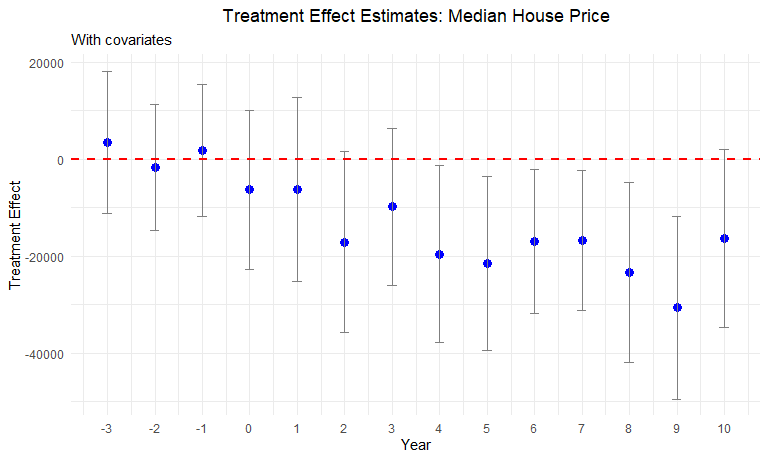
\includegraphics[width=\textwidth,keepaspectratio]{images/tes_gs.png}
    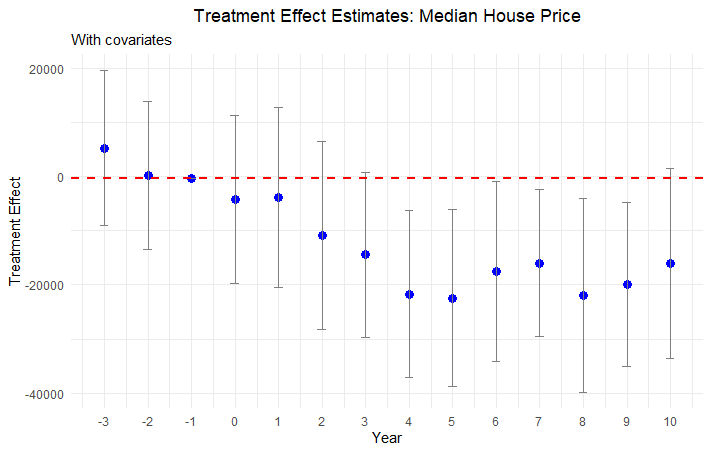
\includegraphics[width=\textwidth,keepaspectratio]{images/tes_gs_reg.png}    
    \caption{Effect plot for Median Housing Price}
    \label{fig:tes_hp}
\end{figure}

Figure \ref{fig:tes_hp} provides an event-study plot that summarizes the treatment effects for each time period. In the graph, we include placebo years up to 3 years before the treatment to show that the median housing prices are statistically identical for cities above and below the threshold prior to the treatment. Each blue dot represents the treatment effect estimate for that year and the bar around it represents the 95\% confidence interval for that estimate. For year 0, which is the year of the vote, we see a slight decrease in the estimate. However, this effect is not statistically significant, as evidenced by the confidence interval containing the null effect. Up to year 3, we observe that the treatment effect estimates are fairly close to zero, and the confidence interval overlaps with zero. As stated previously and shown in Table \ref{tab:median_sale_amount}, we start to see a sizable increase in treatment effect from year 4 onwards and continue to observe it through year 9 after the vote. 
 
\subsection{Heterogeneity Analysis} 

We show the results of our heterogeneity analysis, where we explore the differential impact of cutting road maintenance spending on house prices based on urban vs rural neighborhoods, the size of the tax levy and housing price quantiles.

\vskip 0.5cm

\textbf{Urban vs Rural neighborhoods}: We perform heterogeneity analysis to assess whether different types of neighborhoods and differing size of tax levies result in a differential impact on the housing prices. We first compare urban and rural areas in Ohio. We consider two different ways to define a city as urban:  one including only urbanized areas and another one including both urban areas and urbanized clusters. The event study plot in Figure 6 shows this result. 

\begin{figure}[htbp]
    \centering
    % 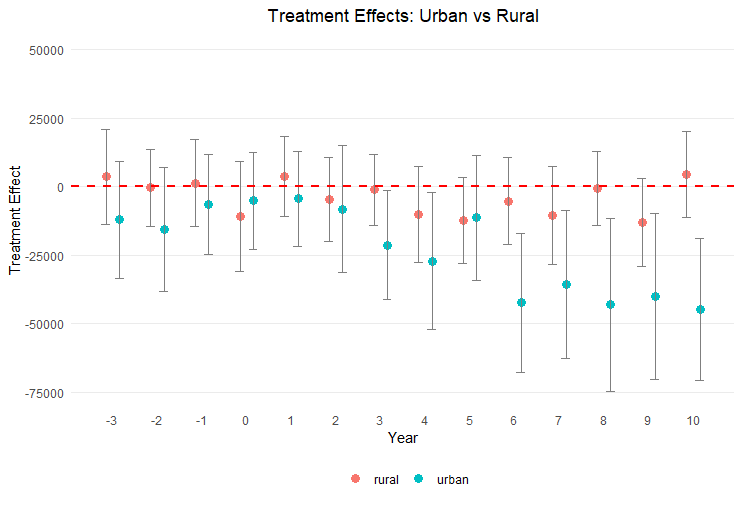
\includegraphics[width=\textwidth,keepaspectratio]{images/tes_covs_ua_new.png}
    % 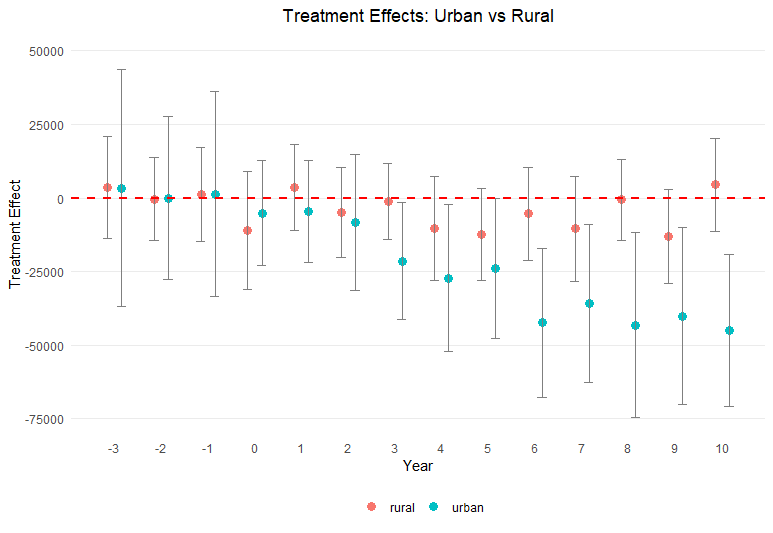
\includegraphics[width=\textwidth,keepaspectratio]{images/tes_covs_ua_clean.png}    
    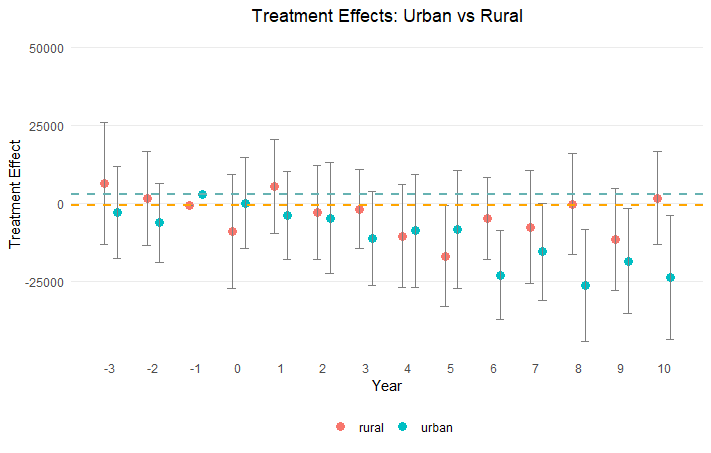
\includegraphics[width=\textwidth,keepaspectratio]{images/tes_covs_ua_reg.png}        
    \caption{Median Housing Price in Urban and Rural Areas}
    \label{fig:tes_covs_ua}
\end{figure}

As shown by Figure \ref{fig:tes_covs_ua}, we do not find any significant differences in housing prices after a renewal tax levy fails to pass for rural areas. On the other hand, we do find a statistically significant decline in housing prices in urban areas starting six years after voting. The standard errors are somewhat smaller for the rural estimates due to a larger number of observations. The difference in point estimates between urban and rural areas may stem from differences in housing supply elasticity (Brasington 2002). Overall, we find that housing prices decrease by \$13,302 on average over the decade\footnote{This is equal to $7.6\% = \frac{13,302}{175,217} \times 100$, where the denominator is average sale price of homes in urban areas in our dataset} after cutting road maintenance tax levies in urban areas. 

\vskip 1cm

\textbf{Tax magnitude}: We check whether the treatment effect is greater for bigger tax levies than smaller tax levies. For this analysis, we split the tax levies based on the millage of a tax levy that is voted upon, where one mill is one tenth of one percent. Mean millage in our dataset is 1.9. We split the data into two parts: small tax levies $\le$ 1.9 mills and large tax levies $>$ 1.9 mills. We do not identify a consistent statistically significant difference in treatment effects between smaller and larger tax levies, suggesting a lack of dose-response. Figure \ref{fig:tes_covs_size} illustrates this result.

\begin{figure}[htbp]
    \centering
    % 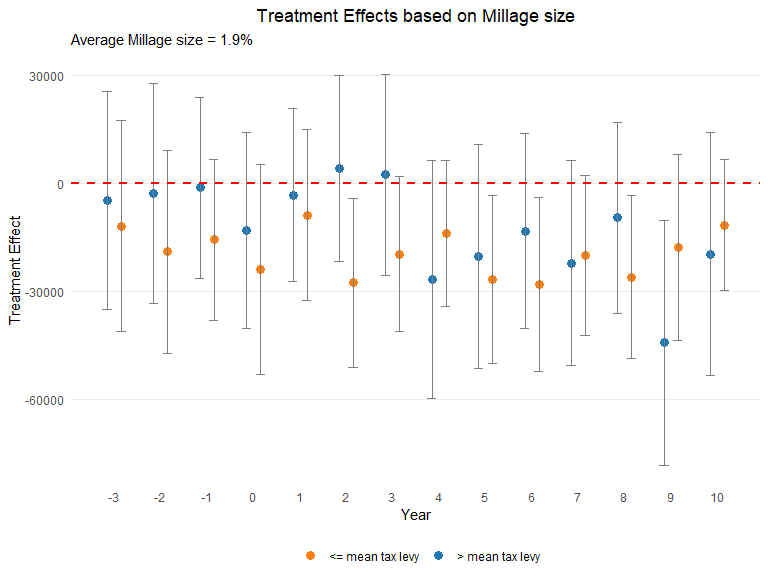
\includegraphics[width=\textwidth,keepaspectratio]{images/tes_size.png}
    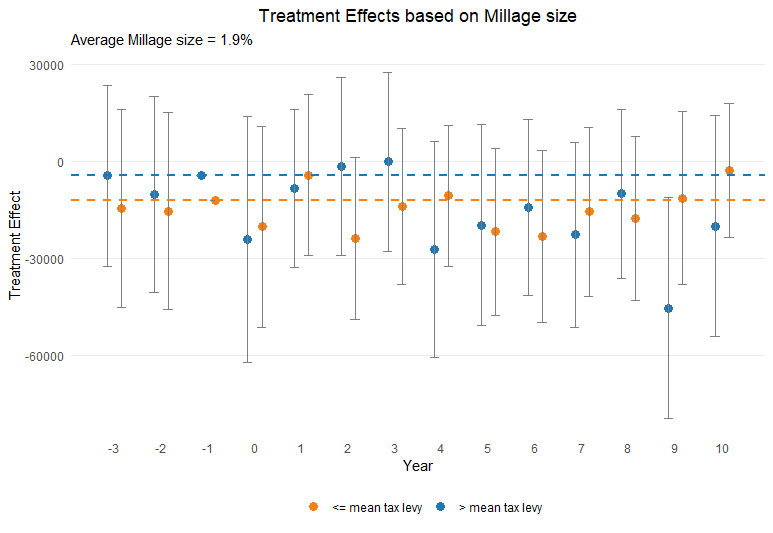
\includegraphics[width=\textwidth,keepaspectratio]{images/tes_size_re.png}    
    \caption{Median Housing Price based on Millage size}
    \label{fig:tes_covs_size}
\end{figure}

All the years before the reduction in road spending have treatment effect estimates with confidence intervals containing zero. Starting in year $t+2$, we observe statistically significant treatment effects in some years after the vote such as year 5, 6 and 8 that show a for tax levies with millage size equal to or below the mean. However, we do not see a consistent decrease in housing prices. Hence, we conclude that the decrease in housing prices of cities that fail to maintain their roads does not vary significantly based on the size of the tax levy.

\vskip 1cm

\textbf{RDD Quantile Estimation}: We further analyze our results by estimating quantile-level treatment effects, as suggested by Frandsen et al (2012), to study how the treatment’s impact varies at different quantiles of the outcome variable. 

\begin{table}[ht]
    \hspace{-1cm}
    % \centering
    \caption{Quantile-level Treatment Effects of Cutting Road Spending on Median House Prices}
    \label{tab:quantile_tes}
    \begin{tabular}{p{1.5cm}ccccccc}
        \hline
        Percentile & $t + 4$ & $t + 5$ & $t + 6$ & $t + 7$ & $t + 8$ & $t + 9$ & $t + 10$ \\
        \hline
        10\% & -6,433 & -22,570 & -9,602 & -12,984 & -11,217 & -6,569 & -1,326 \\
        & (9,364) & (9,065) & (9,205) & (8,420) & (9,136) & (10,809) & (8,793) \\
        20\% & -5,400 & -15,070 & 4,014 & -14,682 & -15,040 & -3,228 & 624 \\
        & (9,983) & (9,886) & (7,443) & (8,502) & (8,160) & (10,435) & (8,509) \\
        70\% & -21,760 & -11,171 & -38,082 & -36,685 & -21,356 & -25,605 & -18,600 \\
        & (12,333) & (11,806) & (12,835) & (12,163) & (12,218) & (13,984) & (9,872) \\
        80\% & -28,478 & -16,379 & -38,460 & -37,470 & -28,950 & -27,800 & -18,658 \\
        & (13,343) & (11,404) & (18,623) & (12,169) & (12,507) & (12,421) & (11,808) \\
        90\% & -51,470 & -34,604 & -38,510 & -27,039 & -29,010 & -49,093 & -36,662 \\
        & (18,409) & (15,837) & (22,194) & (16,308) & (16,640) & (14,498) & (19,110) \\
        \hline
    \end{tabular}
    \begin{tablenotes}
        \small
        \item The outcome is median house price in constant 2010 U.S. dollars. The unit of observation is the city-year, so a treatment effect of -\$28,478 means that at the 80th percentile of house prices four years after the vote, cities that fail to renew road taxes and its associated spending have houses that sell for \$28,478 less than cities that vote to renew road taxes and spending. The regressions include covariates related to the demographics and socioeconomic factors of the cities, drawn from Table \ref{tab:variable_means_sd}.
    \end{tablenotes}
\end{table}

\begin{figure}[htbp]
    \centering
    % 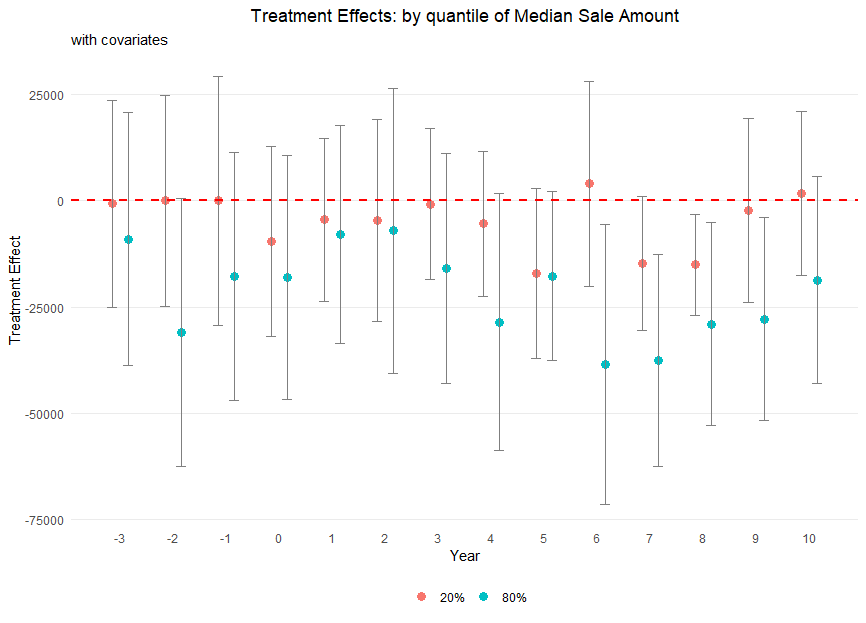
\includegraphics[width=\textwidth,keepaspectratio]{images/tes_qte_covs.png}
    % 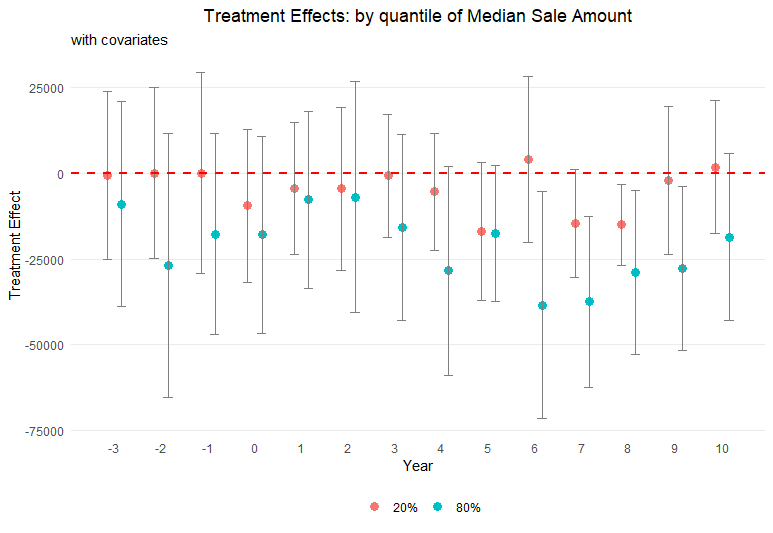
\includegraphics[width=\textwidth,keepaspectratio]{images/tes_qte.png}    
    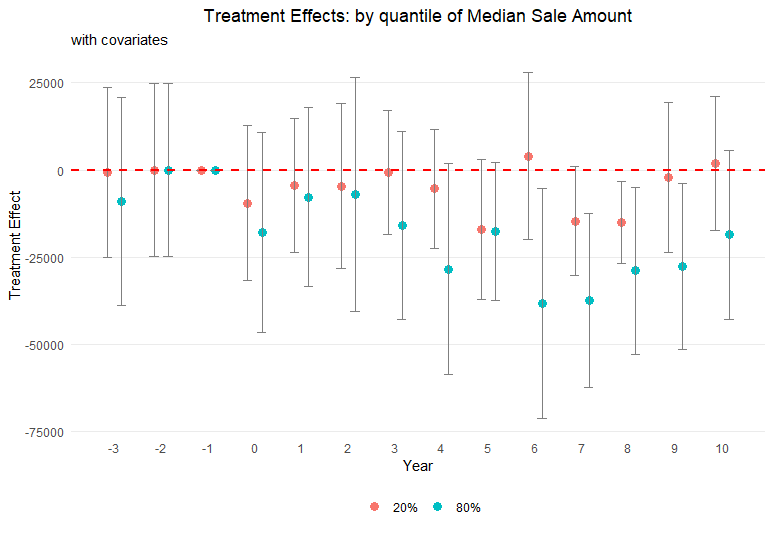
\includegraphics[width=\textwidth,keepaspectratio]{images/tes_qte_re.png}    
    \caption{Median Housing Price based on Quantiles: 20\% and 80\%}
    \label{fig:tes_qte_covs}
\end{figure}

Table \ref{tab:quantile_tes} shows the treatment effect heterogeneity of cutting road spending on high and low quantiles of median house prices. The top percentiles consistently exhibit a statistically significant decline in house sale prices, beginning in year 6 after the reduction in road spending. In contrast, the lower percentiles do not demonstrate a consistent treatment effect. This suggests a differential impact, where higher-valued properties are more sensitive to road disrepair than lower-valued houses. Figure \ref{fig:tes_qte_covs} contrasts the treatment effects of the 20th and 80th percentiles of home sale prices in an effect plot to highlight this differential impact of reduction in road maintenance spending.

\subsection{Robustness Tests}

We conduct several robustness tests to ensure the validity of our results. We test the sensitivity of our results to different bandwidths, covariates, and functional forms. We also check for the presence of pre-trends and perform a placebo test to confirm the validity of our RDD.

\vskip 0.5cm

\textbf{Removing contradictory observations}: In this test, we focus on ensuring the independence and exogeneity of our dataset, a critical aspect in assessing the impact of renewal tax levies on housing prices. An additional concern is the potential bias introduced by tax levies for additional money that might pass after renewal tax levy decisions.
To address this concern, we exclude observations from our analysis if a tax levy for additional funding is introduced and passed within a ten-year period following a renewal tax levy vote. This approach is premised on the notion that the introduction of new funding through additional levies could confound the effects of decreased road taxes on housing prices. 
For example, consider a scenario where a city votes on a renewal tax levy in the year 2000. If that city subsequently introduces and passes a tax levy for additional road spending in 2004, we exclude all votes for that city from 2005 through 2010. This exclusion ensures that the effect on house prices from the 2000 vote are captured for uncontaminated years but not for years after 2004 when the effect of additional road taxes may counteract the drop in tax money from the year 2000 vote. It allows us to isolate and examine the pure impact of the drop in funding from failing renewal levies on housing prices. 

\begin{table}[ht]
    \centering
    \caption{Effect on Median Sale Amount of Failing to Renew a Road Tax Levy}
    \label{tab:uncontaminated}
    \begin{tabular}{p{2.8cm}ccccccc}
        \hline
        year relative to vote & $t + 4$ & $t + 5$ & $t + 6$ & $t + 7$ & $t + 8$ & $t + 9$ & $t + 10$ \\
        \hline
        Treatment effect & -19,015 & -15,609 & -18,403 & -20,842 & -18,950 & -28,634 & -23,823 \\
        standard error   & (9,563) & (10,283) & (10,246) & (9,629) & (9,179) & (7,770)  & (10,594) \\
        Effective bandwidth (h) & 6.88 & 5.92 & 8.36 & 9.42 & 7.91 & 5.43 & 7.05 \\
        Bias bandwidth (b)      & 12.14 & 15.94 & 14.53 & 17.87 & 15.24 & 11.90 & 17.33 \\
        Effective Observations  & 475 & 389 & 561 & 611 & 475 & 300 & 374 \\
        Total Observations      & 2,389 & 2,274 & 2,145 & 2,016 & 1,890 & 1,787 & 1,666 \\
        \hline
    \end{tabular}
    \begin{tablenotes}
        \small
        \item The outcome is median house price in constant 2010 U.S. dollars. The unit of observation is the city-year, so a treatment effect of -\$19,015 means that four years after the vote, cities that fail to renew road taxes and its associated spending have houses that sell for \$19,015 less than cities that vote to renew road taxes and spending. The regressions include covariates related to the demographics and socioeconomic factors of the cities, drawn from Table~\ref{tab:variable_means_sd}.
    \end{tablenotes}
\end{table}


Upon implementing this data filtration, we observe that the treatment effect of the renewal levies on housing prices, measured from $t+1$ to $t+10$, remains largely consistent with our initial findings. This consistency in treatment effect, despite the exclusion of potentially confounding data, lends further credence to our results. The standard errors increase slightly due to reduction in sample size caused by the aforementioned data filtration process. 

\textbf{Placebo cutoffs}: In our primary analysis, the pivotal threshold for the vote share running variable is 50\%, indicating whether a renewal levy passes or fails.  Although we find significant treatment effects using this 50\% threshold, it could be random jumps in the data rather than cutting road taxes and funding that are responsible for the significant estimates.  To this end we conduct a series of placebo tests using alternative cutoffs: 30\%, 40\%, 60\%, and 70\%. Table \ref{tab:placebo_cutoffs} below summarizes the results from the placebo cutoffs analysis. 

\begin{table}[!ht]
    \centering
    \caption{Robust Treatment Effect Estimate for Placebo Cutoffs}
    \label{tab:placebo_cutoffs}
    \begin{tabular}{p{2cm}cccc}
        \hline
        Years after vote & 30\% & 40\% & 60\% & 70\% \\
        \hline
        $t + 4$ & 2,578 & 9,149 & 9,419 & -12,987 \\
                & (8,209) & (7,284) & (11,462) & (14,365) \\
        $t + 5$ & -6,381 & -29,077 & 6,383 & 41,683 \\
                & (9,086) & (20,680) & (10,786) & (17,836) \\
        $t + 6$ & 7,681 & 5,573 & -1,095 & -14,226 \\
                & (9,616) & (8,120) & (8,612) & (15,733) \\
        $t + 7$ & 1,162 & 3,982 & -12,050 & 22,261 \\
                & (10,468) & (8,191) & (9,396) & (19,765) \\
        $t + 8$ & 4,334 & 12,881 & 3,593 & 31,696 \\
                & (9,670) & (8,625) & (10,061) & (6,902) \\
        $t + 9$ & 851 & 7,381 & -6,935 & 42,790 \\
                & (5,921) & (6,333) & (7,114) & (15,663) \\
        $t + 10$ & 10,032 & -35,038 & 324 & -8,566 \\
                 & (10,599) & (35,569) & (8,220) & (17,281) \\
        \hline
    \end{tabular}
    \begin{tablenotes}
        \small
        \item \textit{Notes:} Robust treatment effect estimate for placebo cutoffs as per the estimator from \cite{calonico2017rdrobust}. The unit of observation is city-year level. Standard errors are shown in parentheses below each estimate.
    \end{tablenotes}
\end{table}


Table \ref{tab:placebo_cutoffs} does not show consistently significant treatment effects for any of the placebo cutoffs for our parameter of interest. This absence of significance at thresholds other than the true 50\% reinforces the idea that the effects we observe at the 50\% mark are not a mere coincidence or a result of random variation in the data, but are indeed attributable to the dynamics surrounding the passing or failing of renewal tax levies. 

\textbf{Winsorization}: The debate over whether to include or exclude outliers continues, with some research suggesting that trimming outliers does not improve mean squared error (e.g., Bollinger and Chandra, 2005).  We now drop the 1\% tails to help curtail the influence of outliers. The overall sample mean after dropping 1\% tails is \$144,268 in constant 2010 dollars with a standard deviation of \$109,624. After performing this winsorization step, we re-estimate the treatment effect of failing to renew a road tax levy on housing outcome variables. The results from this estimation process are summarized in Figure \ref{fig:tes_g_w} below:

\begin{figure}[htbp]
    \centering
    % 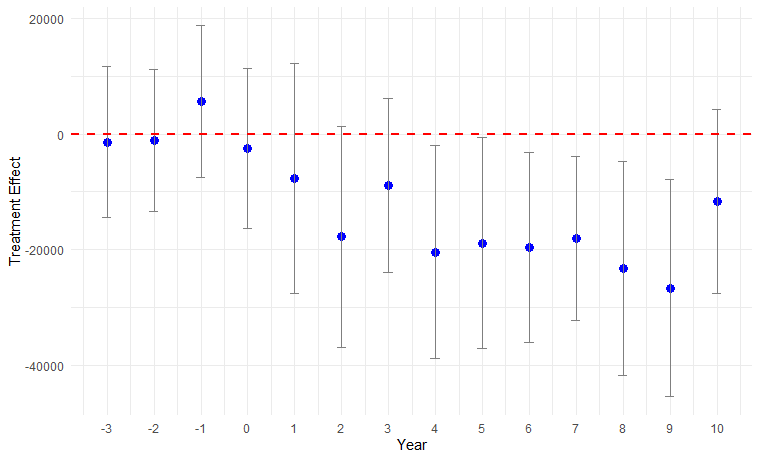
\includegraphics[width=\textwidth,keepaspectratio]{images/tes_g_w.png}
    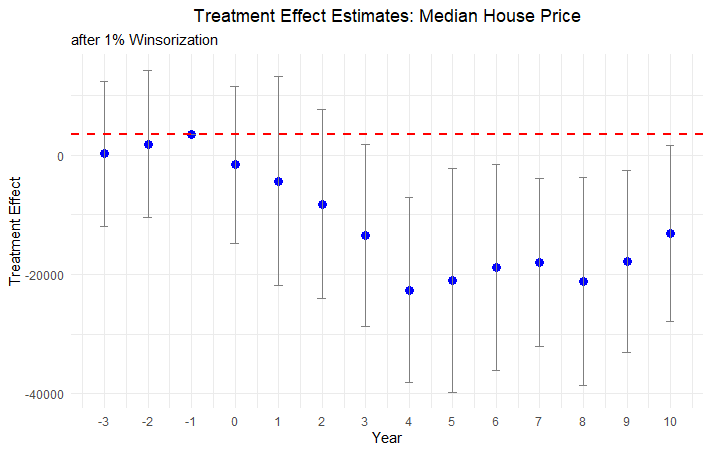
\includegraphics[width=\textwidth,keepaspectratio]{images/tes_g_w_reg.png}    
    \caption{Median Housing Price after 1\% Winsorization}
    \label{fig:tes_g_w}
\end{figure}

The treatment effect estimates with winsorization mimic those from our baseline regression results qualitatively and quantitatively.

\textbf{Covariate Discontinuity}: A fundamental RDD assumption is that observations just above and below the threshold are comparable in all aspects except for treatment status. Table \ref{tab:covariate_discontinuity} presents balance tests across key community characteristics at the voting threshold. As shown, demographic and socioeconomic variables—including population size, poverty rates, educational attainment, employment status, and racial composition—exhibit no statistically significant discontinuities at the cutoff. The absence of any discontinuity suggests that our estimated effects on housing prices represent the impact of failing to renew road tax levies rather than pre-existing community differences. This balance verification via a formal RD test, using covariates as the outcome variable, further strengthens our conclusion that the observed housing price effects stem directly from decisions regarding road tax levies, not from underlying differences in community characteristics.

\begin{table}[!h]
    \centering
    \caption{Covariate Discontinuity Test Results}
    \label{tab:covariate_discontinuity}
    \begin{tabularx}{\textwidth}{l*{3}{X}X}
        \hline
        Variable & Estimate & Standard error & p-value & Confidence interval \\
        \hline
        Population                           & -388      & 1,094   & 0.722  & [-2,532, 1,755] \\
        Poverty Rate                         & 0.017     & 0.014   & 0.234  & [-0.011, 0.045] \\
        \% with Kids                         & -0.007    & 0.012   & 0.539  & [-0.030, 0.015] \\
        \% Households with Children under 18 & 0.0001    & 0.007   & 0.981  & [-0.014, 0.014] \\
        \% Less than High School Education   & -0.004    & 0.020   & 0.834  & [-0.043, 0.035] \\
        \% Some College Education            & -0.012    & 0.011   & 0.274  & [-0.034, 0.009] \\
        \% Unemployment Rate                 & -0.002    & 0.006   & 0.733  & [-0.013, 0.009] \\
        \% Renters                           & -0.005    & 0.015   & 0.754  & [-0.035, 0.025] \\
        \% White                             & -0.007    & 0.011   & 0.499  & [-0.028, 0.014] \\
        \% Black                             & -0.004    & 0.009   & 0.685  & [-0.021, 0.014] \\
        \% Married                           & -0.013    & 0.015   & 0.374  & [-0.042, 0.016] \\
        \% Separated                         & 0.001     & 0.002   & 0.485  & [-0.002, 0.004] \\
        \hline
    \end{tabularx}
    \begin{tablenotes}
        \small
        \item \textit{Notes:} Estimates indicate the treatment effect of failing to renew a road maintenance tax levy on each covariate considered during our study. Confidence intervals are presented in square brackets.
    \end{tablenotes}
\end{table}

\section{Mechanisms} \label{sec:mech}

A key question surrounding our findings is \textit{why} cutting road taxes would lead to a sustained decline in local house prices. In this section, we argue that these results are consistent with classical insights from the literature on local public finance, especially the work of \cite{Tiebout1956} and \cite{Oates1972}. Specifically, cutting road-maintenance tax levies reduces local government funds, which in turn constrains the government’s ability to provide road-upkeep services. This deterioration in road quality then directly and indirectly lowers housing values. Three interconnected channels explain this relationship.

{\bf Road Tax Cuts and Reduced Road Maintenance Funds.} Local governments in Ohio, like those in many other U.S. states, rely on property taxes and dedicated road levies to fund local public goods. The \cite{Oates1972} decentralization theorem highlights that local authorities can generally provide public services in a manner better aligned with resident preferences than would a higher-level government, provided they have adequate revenue sources. When a renewal levy fails at the ballot box, one of these critical revenue sources vanishes. Consistent with the premise that local road quality is a “local public good,” losing a dedicated revenue stream substantially weakens a city’s ability to maintain or upgrade roads. Empirically, we surmise the size of the drop in maintenance funds available to local governments (see Section \ref{tab:levy_stats}). In the spirit of \cite{Tiebout1956}, local residents effectively “vote” on their tax and expenditure bundles, which results in a budgetary contraction. Absent compensating resources from state or federal authorities, the lower tax revenue directly leads to a loss in funding for these local governments, with ripple effects for local roads and infrastructures.

% {\bf Declining Road Quality.} Larger budget constraints produce measurable degradation in road quality. Results from our AI model-based road-quality measure in Section \ref{sec:road_quality_decline} show a marked decrease in road quality following the cessation of renewal levies. The resulting deterioration in road quality may be accompanied by ride discomfort, declining aesthetics, and reduced usability of neighborhood roads. This is precisely what a local public goods framework would predict: fewer financial resources for upkeep immediately impact the daily “consumption” of roads. Residents observe these changes slowly over time, often after four to five years, before road conditions become visibly poor.

{\bf Declining Road Quality.} Results from our AI model-based road-quality measure in Section \ref{sec:road_quality_decline} show a marked decrease in road quality following the cessation of renewal levies. The resulting deterioration in road quality may be accompanied by ride discomfort, declining aesthetics, and reduced usability of neighborhood roads. This is precisely what a local public goods framework would predict: fewer financial resources for upkeep immediately impact the daily “consumption” of roads. Residents observe these changes slowly over time, often after four to five years, before road conditions become visibly poor.

{\bf Capitalization into house Prices.} Falling road quality imposes a disamenity on local residents. As recognized by \cite{Oates1969}, property values in a community incorporate expectations of both the level of taxation and the quality of local services. While homebuyers benefit from understanding they might pay lower property taxes in a municipality with a failing levy, they also factor in the anticipated (and eventually realized) deterioration of roads. Several mechanisms help explain the ultimate discount in property values:

\begin{enumerate}
    \item \textbf{Appearance and Neighborhood Appeal.} Rough roads, potholes, and poorly patched surfaces reduce aesthetic appeal. Potential buyers, seeing visible signs of neglect, bid less.
    \item \textbf{Vehicle Damage and Travel Costs.} Chronic maintenance problems translate into higher expenditures on tires, suspensions, and alignments, as well as more time lost to slower commutes.
    \item \textbf{Expectation of Reduced Public Services.} A failed renewal levy may signal broader fiscal stringency, causing residents to expect other future service cutbacks. Uncertainty about service levels weighs negatively on property values. 
\end{enumerate}

\noindent In this sense, the local “bundling” of taxes and roads is priced into real estate transactions, echoing the original proposition of \cite{Tiebout1956} that local public goods are \emph{capitalized} in property values. Our event-study evidence confirms that the negative price effects are most pronounced several years after the renewal levy fails, consistent with the time needed for visible road quality decline to become salient to homeowners and prospective buyers.

{\bf Short-Run versus Long-Run Trade-Off.} Importantly, a trade-off emerges over time. In the short run, residents who voted down the road tax levy experience immediate relief in terms of lower property tax bills. Their out-of-pocket expenses decline, which can be a tangible financial benefit—particularly in communities where property tax burdens were already viewed as high. However, as road quality starts to visibly deteriorate from around the fourth year onward (see \ref{tab:median_sale_amount}), the same residents find themselves negatively affected by a decline in house prices. This lag reflects the time it takes for infrastructure disrepair to become apparent, be it through more frequent potholes or visibly eroding surfaces. By the time these problems are indisputable, the neighborhood’s real-estate market has had sufficient time to register the disamenity, capitalizing it as a discount in property values. This dynamic captures a fundamental insight of local public finance: the preferences of current taxpayers can diverge from the longer-term public interest \citep{BuchananTullock1962, AlesinaTabellini1990}. While voters may respond to short-term cost savings from a failing levy, the forgone maintenance ultimately reduces the community’s appeal and leads to diminished investment returns—particularly for homeowners whose largest asset is their property. Hence, the immediate reduction in tax liabilities ultimately collides with the reality of lower market valuations once inadequate road upkeep becomes plainly visible.

% \bigskip

In summary, our findings align with longstanding theories of local public finance. Under the logic proposed by \cite{Oates1972}, letting local jurisdictions decide on road tax levies can promote efficient provision of local services, as long as there is sufficient willingness among residents to sustain the quality of road infrastructure. However, once communities choose (either inadvertently or intentionally) to forgo a renewal levy, the immediate loss of funds and subsequent lagged deterioration in road quality erode property values. From the household’s perspective, subpar road maintenance becomes an undesirable aspect of the local package they are effectively “purchasing” when buying a home, leading to a downward shift in housing demand—and hence, in median home sale prices.

% \section{Mechanisms} \label{sec:mech}

% The central finding of our paper is that local governments experiencing road-tax renewal failures see significant declines in road quality and, subsequently, in housing prices. This section outlines the channels driving this result and connects each to seminal works in infrastructure economics, property valuation, and public finance. Specifically, we discuss: (i) the loss of dedicated revenue streams following failed levies, (ii) the consequent under-provision of road maintenance and deterioration in road quality, and (iii) how poor road quality translates to lower home prices through both functional and perceptual channels.

% \subsection*{1. Reduced Revenue and Under-Provision of Road Maintenance}

% A robust body of literature links infrastructure spending to local economic well-being. \cite{Gramlich1994} underscores how local infrastructure—particularly roads—directly contributes to both residential welfare and business productivity. Once renewal levies fail, municipalities face immediate budgetary shocks, losing earmarked resources for critical repairs and upkeep. Without a guaranteed funding stream, local officials must divert or reduce spending on maintenance and preventative work, creating cumulative disinvestment in road quality over time.

% Budget constraints in local governance often manifest as under-provision of public goods \citep{Fischel2001}, as policymakers are compelled to reallocate limited resources toward other essential services (e.g., law enforcement or general administration). In practice, road maintenance often succumbs to a “defer and patch” strategy that prioritizes urgent fixes at the expense of comprehensive resurfacing projects—resulting in highly visible, steadily worsening road quality.

% \subsection*{2. Physical and Perceptual Decline in Road Quality}

% The deterioration that follows reduced funding is rarely instantaneous; roads degrade gradually, as evidenced by our event-study results. Several scholars note that local infrastructure’s physical depreciation can be slow at first but accelerates without timely maintenance \citep{HoltzEakin1993, Haughwout2002}. In the context of roads, delayed repairs lead to potholes, structural cracks, and uneven surfaces—conditions that, if not remedied, compound into more significant damage requiring costlier interventions down the road.

% Beyond the purely physical aspects, visible degradation fosters negative perceptions of the area among residents and potential homebuyers. The “Homevoter Hypothesis” \citep{Fischel2001} suggests that homeowners, motivated by protecting their property values, closely monitor local government decisions on infrastructure. When they observe (or anticipate) reduced road upkeep, perceptions of overall municipal performance suffer. The resulting belief that road quality will continue to decline can further depress local demand for housing, intensifying the price discount we observe.

% \subsection*{3. Channels Linking Poor Road Quality to Lower Housing Prices}

% \paragraph{(a) Hedonic Valuations.}
% Drawing on the hedonic pricing framework popularized by \cite{Rosen1974}, property values reflect not just the structural characteristics of a home but also neighborhood amenities and disamenities. Deteriorating roads represent a disamenity for multiple reasons: rough driving surfaces impose higher vehicle maintenance costs, commuting is more stressful, and “curb appeal” declines. These factors systematically lower households’ willingness to pay.

% \paragraph{(b) Capitalized Costs and Risks.}
% Local property values incorporate expectations about future taxes and service quality. When road repairs lag, future homeowners anticipate having to pay for tire damage or extra car maintenance, or facing the risk of new, ad-hoc taxation to address infrastructure crises. Such factors become “capitalized” in the purchase price \citep{Brueckner1982}, effectively lowering home valuations if roads are perceived to be underfunded long-term.

% \paragraph{(c) Spatial Externalities and Commuting Costs.}
% Infrastructure scholars such as \cite{HoltzEakin1993} and \cite{Henderson1985} emphasize how higher commuting costs—both monetary and time—reduce the net economic and social benefits of living in certain locations. Poorly maintained local roads amplify these commuting costs, creating a spatial externality that depresses housing demand in neighborhoods where households are likely to endure extra delays or auto-repair expenses.

% \subsection*{Putting It All Together}

% Taken as a whole, these findings present a consistent narrative:
% \begin{enumerate}
%     \item \textbf{Failed levies reduce dedicated funds}, forcing municipalities to cut back on road upkeep or shift limited resources to only the most dire repair tasks.
%     \item \textbf{Road quality gradually declines}, becoming salient to both current and prospective residents, who witness an accumulation of infrastructure problems over multiple years.
%     \item \textbf{Housing prices adjust downward} to reflect new expectations regarding the area’s long-run road conditions, vehicle upkeep costs, and the diminished overall attractiveness of the neighborhood.
% \end{enumerate}

% Importantly, there is a trade-off in the timing of these costs and benefits. In the short run, many residents see an immediate decrease in their out-of-pocket tax expenses when a renewal levy fails. However, as road quality visibly deteriorates over the following years, the longer-term consequence is a decline in neighborhood desirability and thus a drop in house values. This pattern aligns with our empirical finding of significant negative effects on property prices emerging four to five years after a failed road levy vote.

% The lagged effect in house-price reductions aligns with a slower physical manifestation of infrastructure neglect—first, roads appear slightly worn, but only after multiple seasons of continued disinvestment do they exhibit chronic issues that clearly register to prospective homeowners. Buyers and sellers factor these accumulating signals into their transactions, producing the persistent price discount observable several years after the levy failure.

% \bigskip

% In sum, once a road-maintenance levy fails, the structural decline in local infrastructure—both physical and perceptual—becomes a local disamenity capitalized into home values. Seminal scholarship on infrastructure economics and hedonic pricing helps frame how lower road quality translates into reduced property demand, confirming our empirical findings.

\section{Conclusion} \label{sec:conclusion}

A great deal of existing research has focused on the effect of new roads on house prices, especially in developing nations, providing valuable policy insights and spurring development initiatives like China’s Belt \citep{huang2016understanding} and Road Initiative and India’s Pradhan Mantri Gram Sadak Yojana \citep{asher2020}. However, the endogeneity of road placement makes it difficult to identify causal effects. In this paper, we study taxes that fund maintenance of existing roads and avoid endogeneity issues by utilizing a quasi-experiment setting that naturally arises from the voted levies enacted by local governments in Ohio. We study more than 3,000 referendums raised by cities, villages, and townships to renew local road taxes funding existing roads and use ITT RD estimator inspired by \cite{cellini2010value} to estimate the effect of failure to renew a levy on housing prices. We also compute the loss in funding experienced by local governments when they face a tax cut due to failure of a renewal tax levy and fine-tune a Vision Transformer model to predict and identify the changes in road quality in these areas. We find an average decline of 15\% in road quality in areas that cut their renewal taxes and a decline in home sale price of 9\% over the 10-year period. We find no anticipation effects, unlike \cite{beenstock2016hedonic} and \cite{diao2017spatial}, but we find statistically significant effects starting four years and continuing onto the later years. We find these effects to be more consistent for urban rather than rural areas. We find a lack of dose-response based on the size of the levy, but we find larger house price reductions for more expensive houses than for cheaper houses.  

\noindent Future research could extend the dynamic regression discontinuity identification strategy we employ to other geographies, using vote share as a running variable for places that vote on road spending, or using time as a running variable for cities that directly change road spending without a referendum. Moreover, it could also shift away from studying votes to maintain spending toward studying votes to increase road spending, although the endogeneity of choosing when to propose such a referendum makes identification for such settings more challenging.




% \section{Discussions} \label{sec:discussion}

% \section{Conclusion} \label{sec:conclusion}

\singlespacing
\setlength\bibsep{0pt}
\bibliographystyle{aea}
% \bibliography{Placeholder}

\bibliography{aej_references}

\clearpage

\appendix
\section*{Appendix} \label{sec:appendix}
\section{Additional Treatment Effects Tables \& Effect Plots} \label{sec:appxa}

\subsection{Full set of Treatment Effects for Housing Prices}

The full set of treatment effects provided in Table \ref{tab:median_sale_amount_full} support Table \ref{tab:median_sale_amount} which provides treatment effects for the housing price outcome variable in the main body of the paper. These treatment effects are estimated using a regression model that controls for various factors.

\begin{table}[htbp]
    \centering
    \caption{Full set of estimates - Median Housing Price}
    \label{tab:median_sale_amount_full}
    \begin{tabular}{p{3cm}cccc}
        \hline
        \textbf{Year relative to vote} & \textbf{Estimate} & \textbf{Standard error} & \textbf{p-value} & \textbf{Confidence interval} \\
        \hline
        $t - 3$  & 3,468   & 7,465  & 0.642  & [-11,164, 18,099] \\
        $t - 2$  & -1,703  & 6,617  & 0.797  & [-14,673, 11,267] \\
        $t - 1$  & 1,784   & 6,950  & 0.797  & [-11,838, 15,407] \\
        $t + 1$ & -6,197  & 9,662  & 0.521  & [-25,134, 12,741] \\
        $t + 2$ & -17,059 & 9,518  & 0.073  & [-35,715, 1,597] \\
        $t + 3$ & -9,823  & 8,244  & 0.233  & [-25,981, 6,335] \\
        $t + 4$ & -19,535 & 9,289  & 0.035  & [-37,741, -1,329] \\
        $t + 5$ & -21,531 & 9,147  & 0.019  & [-39,459, -3,604] \\
        $t + 6$ & -16,994 & 7,558  & 0.025  & [-31,809, -2,180] \\
        $t + 7$ & -16,991 & 7,357  & 0.023  & [-31,111, -2,272] \\
        $t + 8$ & -23,323 & 9,449  & 0.014  & [-41,842, -4,803] \\
        $t + 9$ & -30,620 & 9,586  & 0.001  & [-49,408, -11,833] \\
        $t + 10$ & -16,411 & 9,342  & 0.079  & [-34,721, 1,898] \\
        \hline
    \end{tabular}
    \begin{tablenotes}
        \small
        \item Supplements Table \ref{tab:median_sale_amount} in text. Full set of treatment effect estimates of renewing road tax levies relative to cutting road tax levies from 3 years before the vote to 10 years after the vote. Covariates from Table \ref{tab:variable_means_sd} used in all regressions. Outcome is median house price in constant 2010 U.S. dollars. Unit of observation is the city-year. A treatment effect of -\$19,535 means that four years after the vote, cities that vote to cut road taxes and its associated spending have houses that sell for \$19,535 less than cities that vote to renew road taxes and spending.
    \end{tablenotes}
\end{table}

\begin{figure}[htbp]
    \centering
    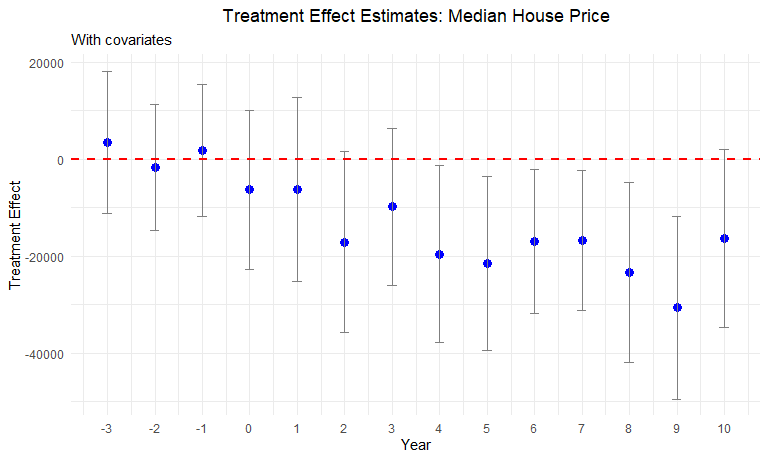
\includegraphics[width=\textwidth,keepaspectratio]{images/tes_gs.png}
    \caption{Event Study - Median Housing Price}
    \label{fig:tes_gs_app}
\end{figure}

\clearpage


% \subsection{Outcome vs Running variable plots for years after Treatment}

\clearpage

\section{Additional Robustness Tests} \label{sec:appxb}

\subsection{Covariate Discontinuity Tests \& Smoothness Plots}

\begin{table}[!h]
    \centering
    \caption{Covariate Discontinuity Test Results}
    \label{tab:covariate_discontinuity}
    \begin{tabular}{p{2cm}cccc}
        \hline
        Variable & Estimate & Standard error & p-value & Confidence interval \\
        \hline
        Population                           & -388      & 1,094   & 0.722  & [-2,532, 1,755] \\
        Poverty Rate                         & 0.017     & 0.014   & 0.234  & [-0.011, 0.045] \\
        \% with Kids                         & -0.007    & 0.012   & 0.539  & [-0.030, 0.015] \\
        \% Households with Children under 18 & 0.0001    & 0.007   & 0.981  & [-0.014, 0.014] \\
        \% Less than High School Education   & -0.004    & 0.020   & 0.834  & [-0.043, 0.035] \\
        \% Some College Education            & -0.012    & 0.011   & 0.274  & [-0.034, 0.009] \\
        \% Unemployment Rate                 & -0.002    & 0.006   & 0.733  & [-0.013, 0.009] \\
        \% Renters                           & -0.005    & 0.015   & 0.754  & [-0.035, 0.025] \\
        \% White                             & -0.007    & 0.011   & 0.499  & [-0.028, 0.014] \\
        \% Black                             & -0.004    & 0.009   & 0.685  & [-0.021, 0.014] \\
        \% Married                           & -0.013    & 0.015   & 0.374  & [-0.042, 0.016] \\
        \% Separated                         & 0.001     & 0.002   & 0.485  & [-0.002, 0.004] \\
        \hline
    \end{tabular}
    \begin{tablenotes}
        \small
        \item Estimates indicate the treatment effect of failing to renew a road maintenance tax levy on each covariate considered during our study. Confidence intervals are presented in square brackets.
    \end{tablenotes}
\end{table}

% \subsection{Covariate Smoothness Plots}

\begin{figure}[ht]
    \centering
    \begin{minipage}[b]{0.40\textwidth}
        \centering
        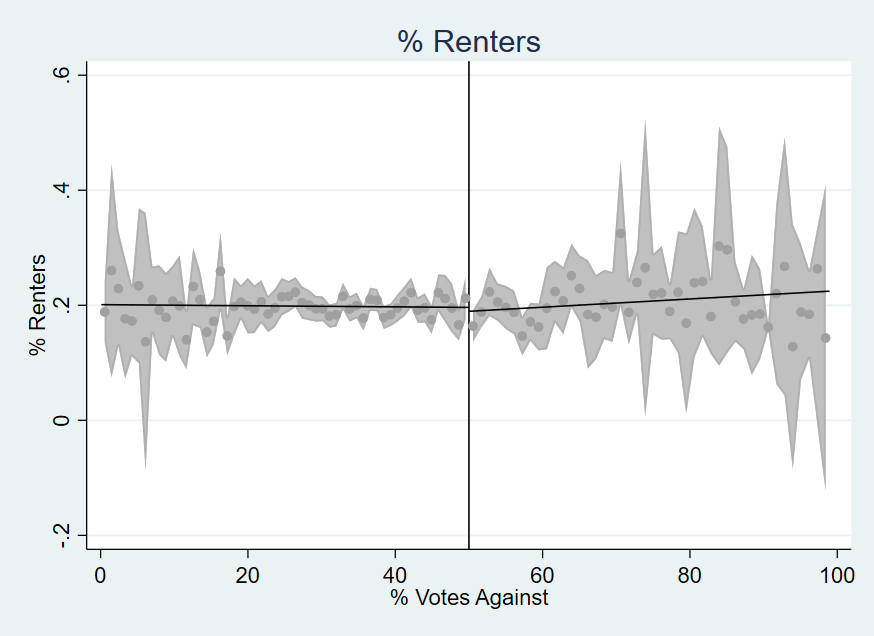
\includegraphics[width=\textwidth,keepaspectratio]{images/cov_smoothness_pctrent.png}
        \caption*{Pct Rent}
        \label{fig:pctrent_sm}
    \end{minipage}
    \hfill
    \begin{minipage}[b]{0.40\textwidth}
        \centering
        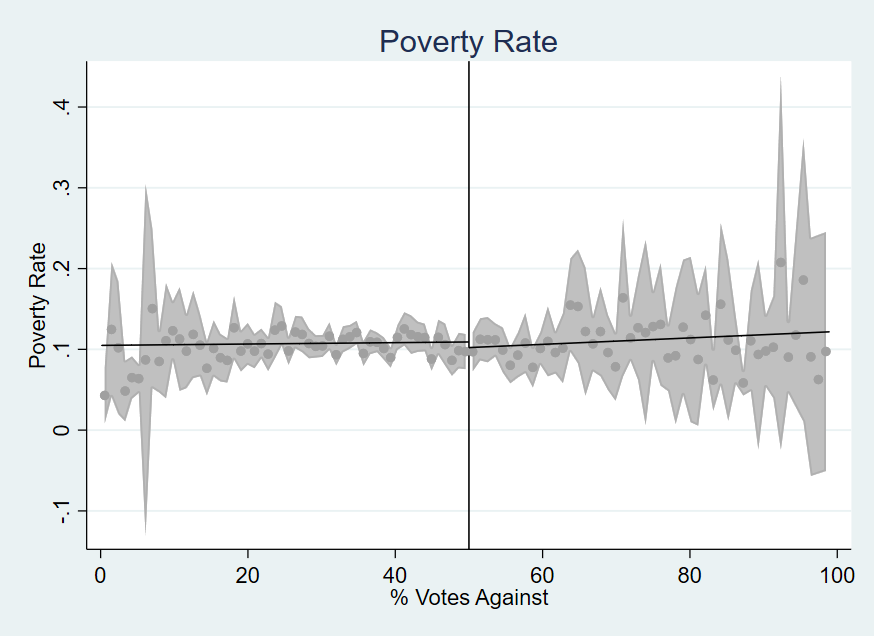
\includegraphics[width=\textwidth,keepaspectratio]{images/cov_smoothness_poverty.png}
        \caption*{Poverty Rate}
        \label{fig:poverty_sm}
    \end{minipage}
    
    % \vspace{1em}
    
    \begin{minipage}[b]{0.40\textwidth}
        \centering
        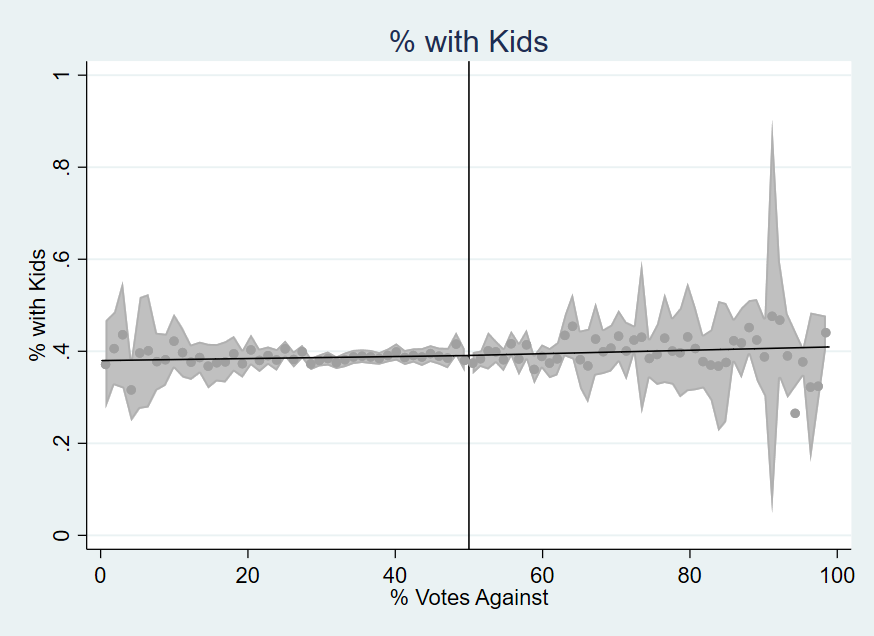
\includegraphics[width=\textwidth,keepaspectratio]{images/cov_smoothness_pctwithkids.png}
        \caption*{Pct With Kids}
        \label{fig:pct_with_kids_sm}
    \end{minipage}
    \hfill
    \begin{minipage}[b]{0.40\textwidth}
        \centering
        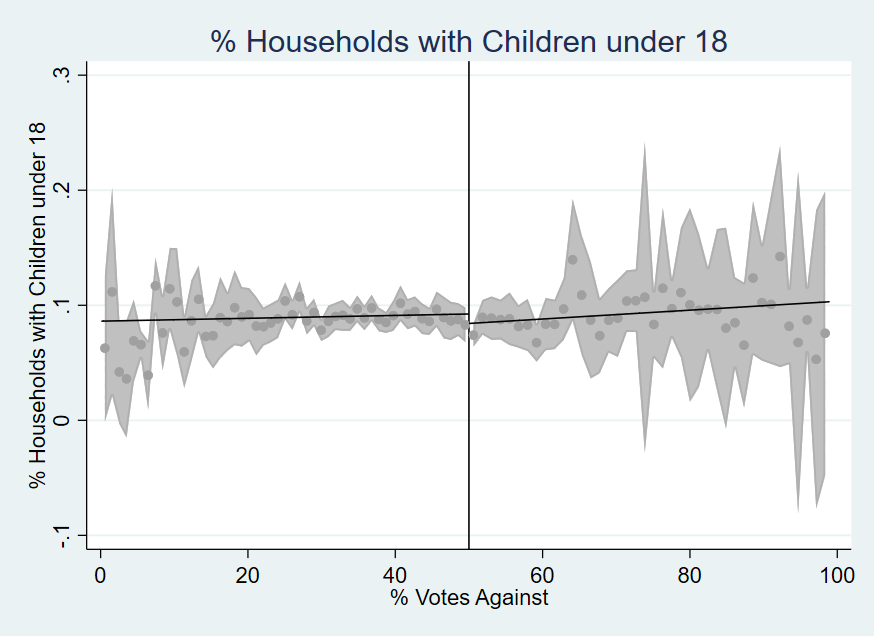
\includegraphics[width=\textwidth,keepaspectratio]{images/cov_smoothness_pctsinparhhld.png}
        \caption*{Pct Single Parent Hhld}
        \label{fig:pctsinparhhld_sm}
    \end{minipage}
    
    % \vspace{1em}
    
    \begin{minipage}[b]{0.40\textwidth}
        \centering
        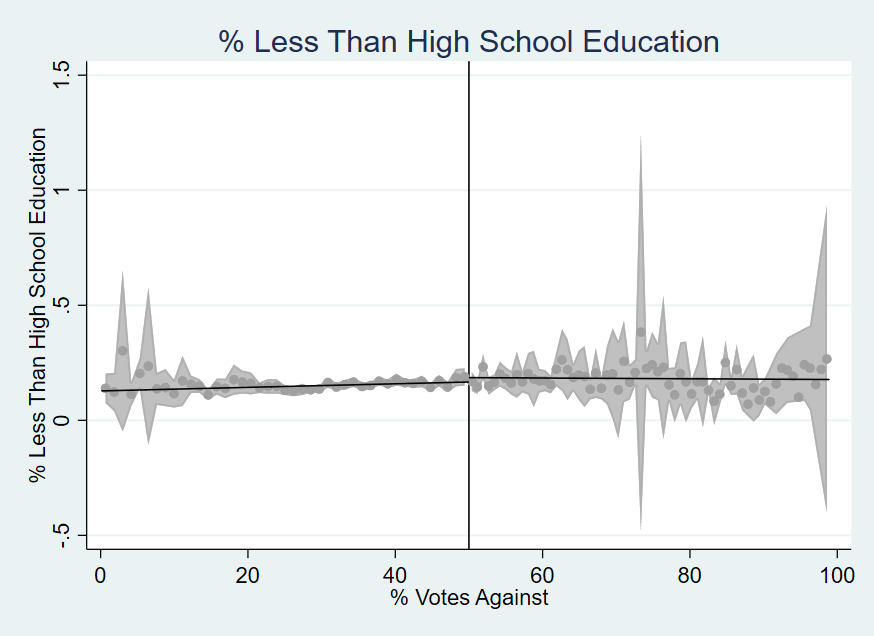
\includegraphics[width=\textwidth,keepaspectratio]{images/cov_smoothness_pctlesshs.png}
        \caption*{Pct Less than HS}
        \label{fig:pctlesshs_sm}
    \end{minipage}
    \hfill
    \begin{minipage}[b]{0.40\textwidth}
        \centering
        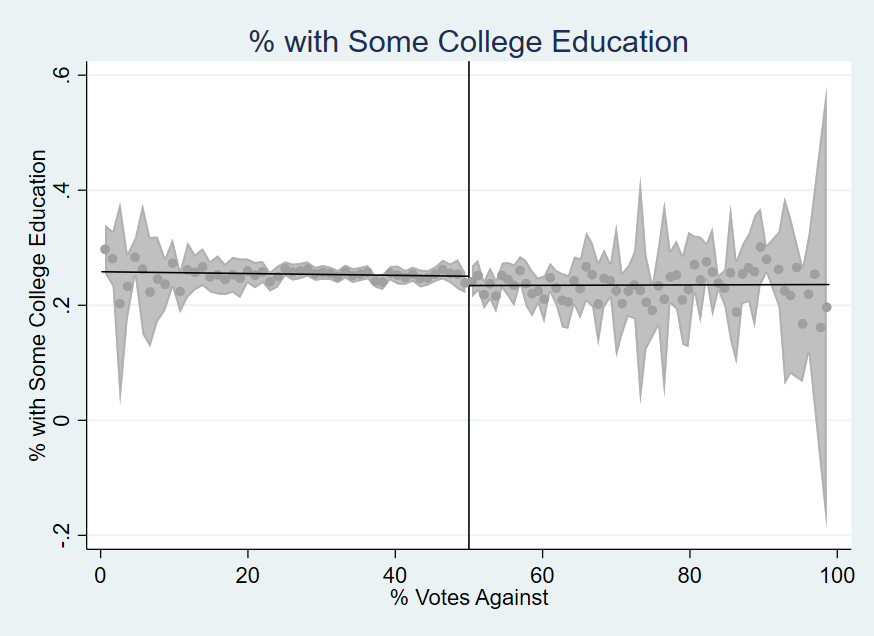
\includegraphics[width=\textwidth,keepaspectratio]{images/cov_smoothness_pctsomecoll.png}
        \caption*{Pct Some College}
        \label{fig:pctsomecoll_sm}
    \end{minipage}
    
    % \vspace{1em}
    
    \begin{minipage}[b]{0.40\textwidth}
        \centering
        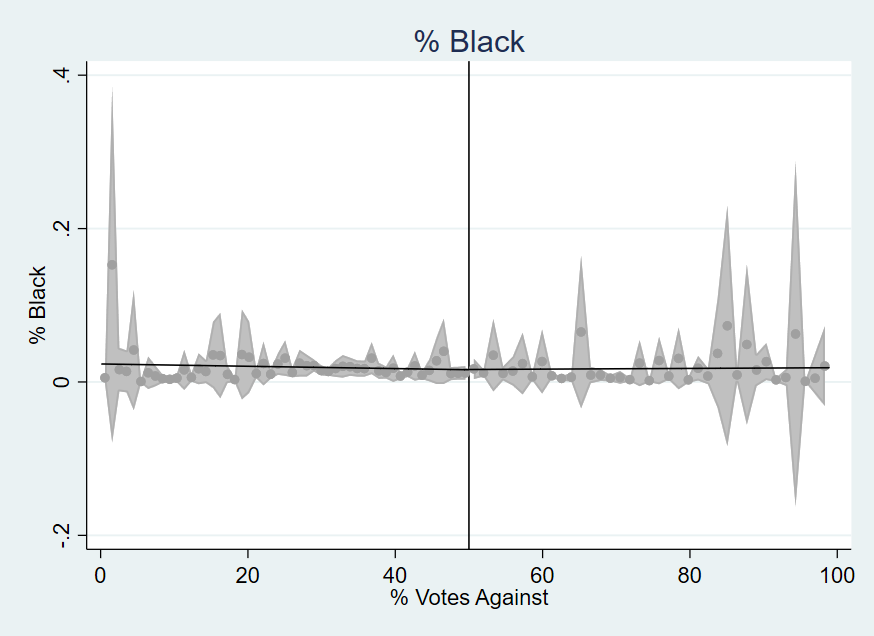
\includegraphics[width=\textwidth,keepaspectratio]{images/cov_smoothness_pctblack.png}
        \caption*{Pct Black}
        \label{fig:black_sm}
    \end{minipage}
    \hfill
    \begin{minipage}[b]{0.40\textwidth}
        \centering
        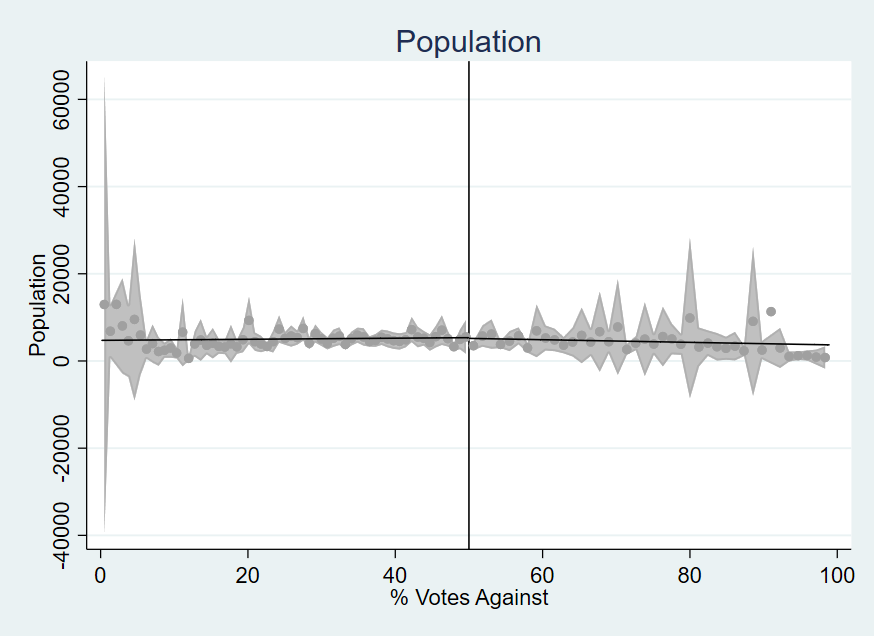
\includegraphics[width=\textwidth,keepaspectratio]{images/cov_smoothness_pop.png}
        \caption*{Population}
        \label{fig:pop_sm}
    \end{minipage}
    
    \caption{Covariate Discontinuity Plots - Part 1}
    \label{fig:rd_cov_smoothness_1}
\end{figure}

\begin{figure}[ht]
    \centering
    \begin{minipage}[b]{0.40\textwidth}
        \centering
        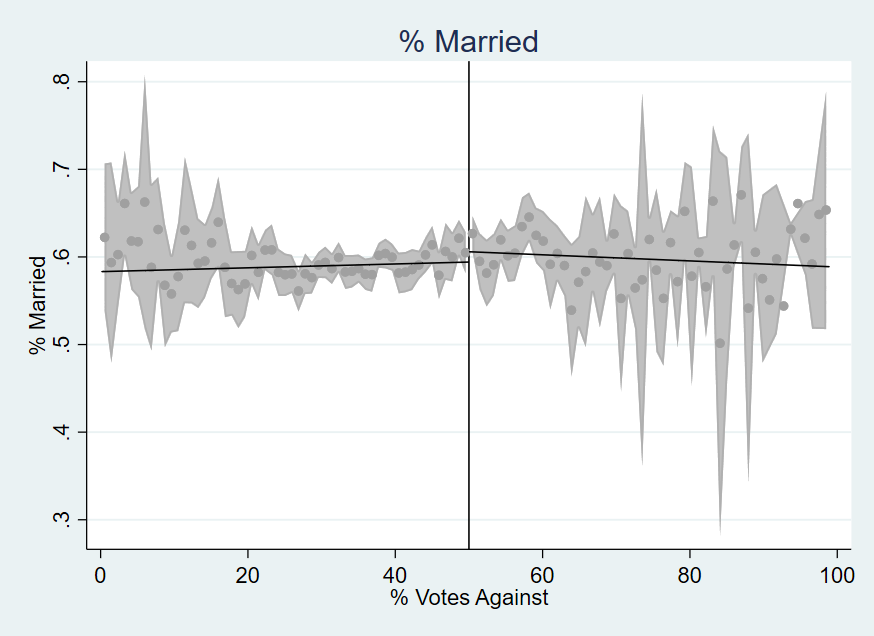
\includegraphics[width=\textwidth,keepaspectratio]{images/cov_smoothness_pctmarried.png}
        \caption*{Pct Married}
        \label{fig:pctmarried_sm}
    \end{minipage}
    \hfill
    \begin{minipage}[b]{0.40\textwidth}
        \centering
        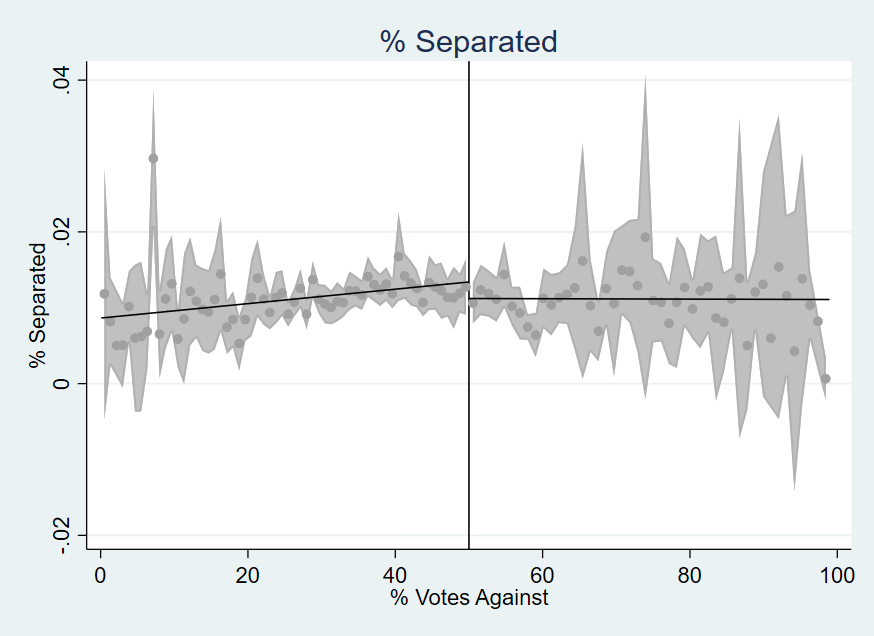
\includegraphics[width=\textwidth,keepaspectratio]{images/cov_smoothness_pctseparated.png}
        \caption*{Pct Separated}
        \label{fig:pctseparated_sm}
    \end{minipage}
    
    \vspace{1em}
    
    \begin{minipage}[b]{0.40\textwidth}
        \centering
        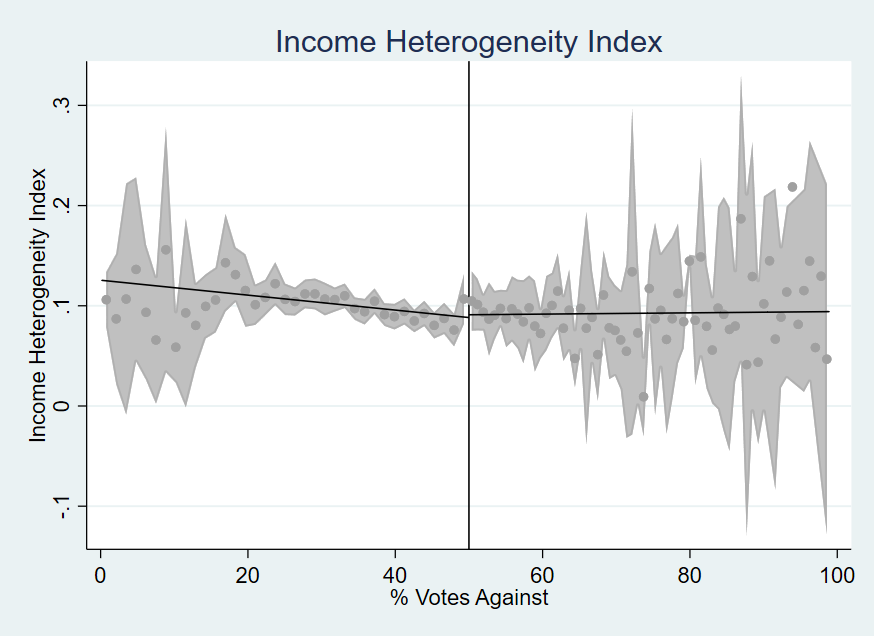
\includegraphics[width=\textwidth,keepaspectratio]{images/cov_smoothness_incherfindahl.png}
        \caption*{Income Herfindahl Index}
        \label{fig:incherfindahl_sm}
    \end{minipage}
    \hfill
    \begin{minipage}[b]{0.40\textwidth}
        \centering
        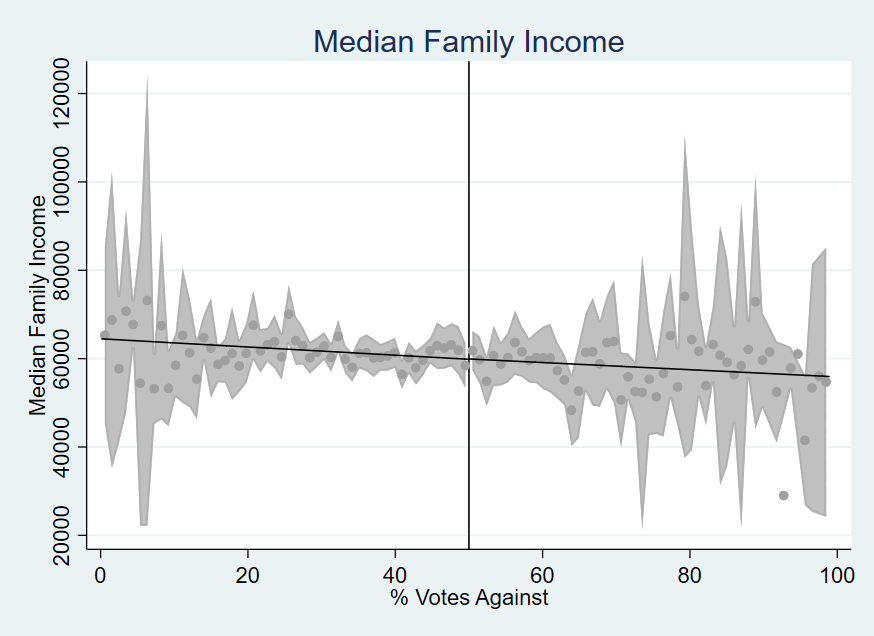
\includegraphics[width=\textwidth,keepaspectratio]{images/cov_smoothness_medfamy.png}
        \caption*{Median Family Income}
        \label{fig:medfamy_sm}
    \end{minipage}
    
    \vspace{1em}
    
    \begin{minipage}[b]{0.40\textwidth}
        \centering
        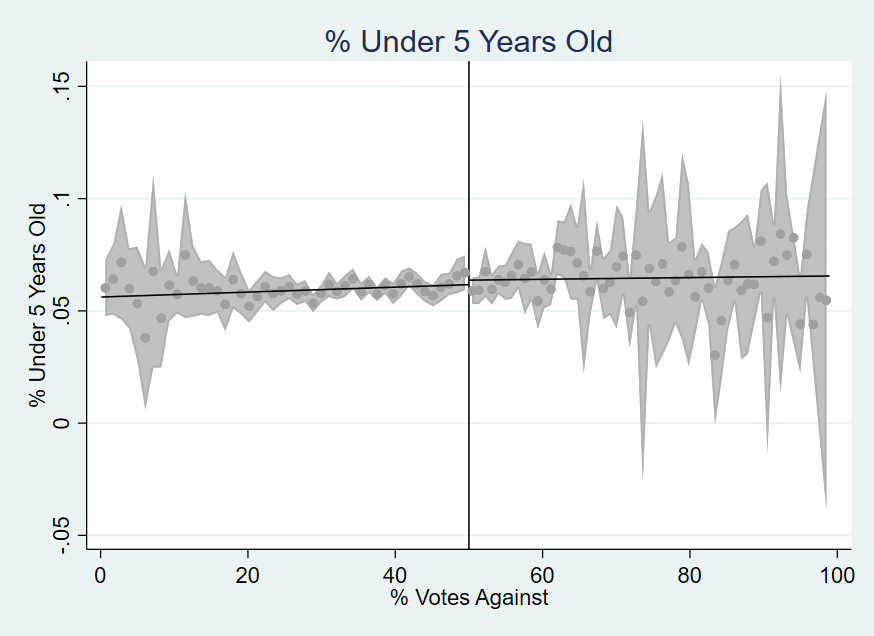
\includegraphics[width=\textwidth,keepaspectratio]{images/cov_smoothness_pctlt5.png}
        \caption*{Pct Less than 5}
        \label{fig:pctlt5_sm}
    \end{minipage}
    \hfill
    \begin{minipage}[b]{0.40\textwidth}
        \centering
        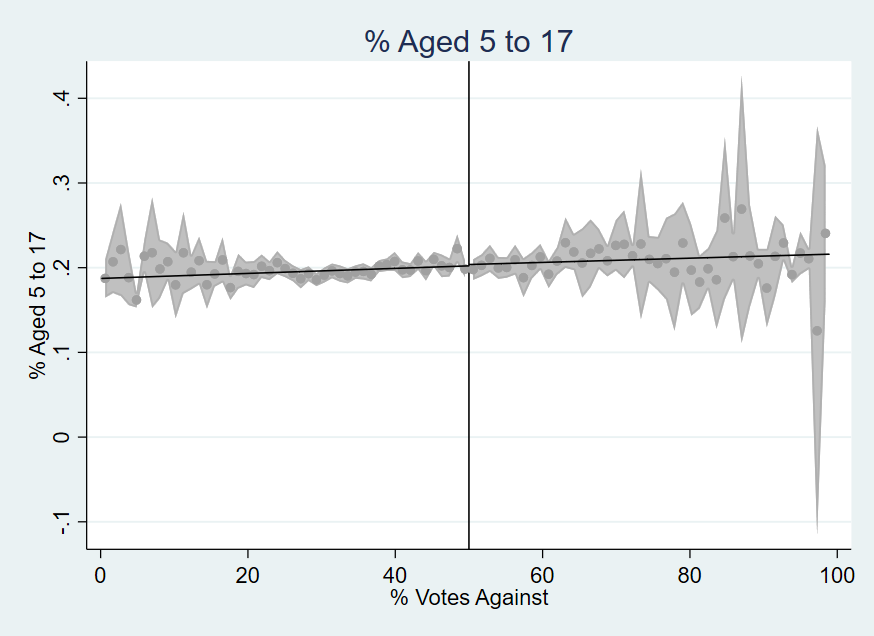
\includegraphics[width=\textwidth,keepaspectratio]{images/cov_smoothness_pct5to17.png}
        \caption*{Pct 5 to 17}
        \label{fig:pct5to17_sm}
    \end{minipage}
    
    \vspace{1em}
    
    \begin{minipage}[b]{0.40\textwidth}
        \centering
        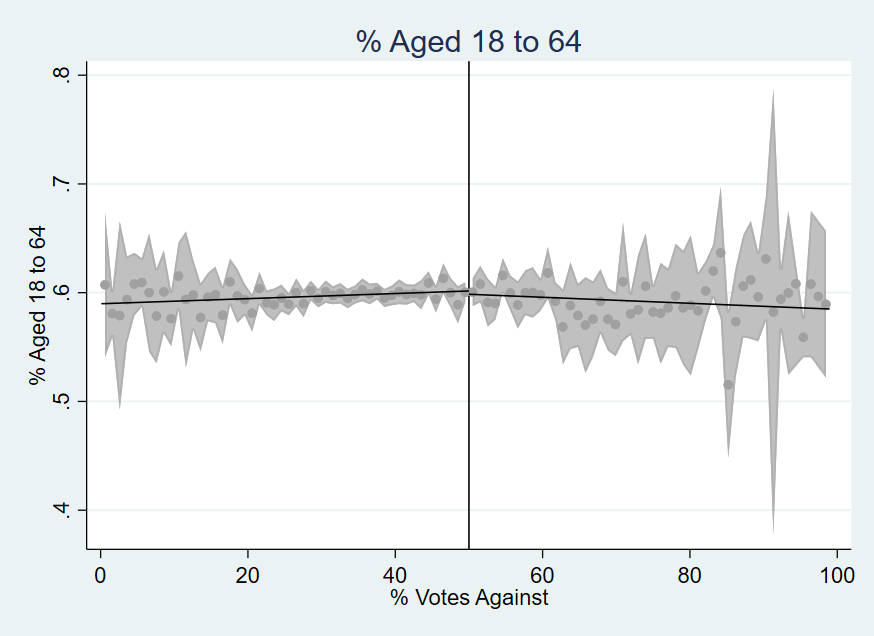
\includegraphics[width=\textwidth,keepaspectratio]{images/cov_smoothness_pct18to64.png}
        \caption*{Pct 18 to 64}
        \label{fig:pct18to64_sm}
    \end{minipage}
    \hfill
    \begin{minipage}[b]{0.40\textwidth}
        \centering
        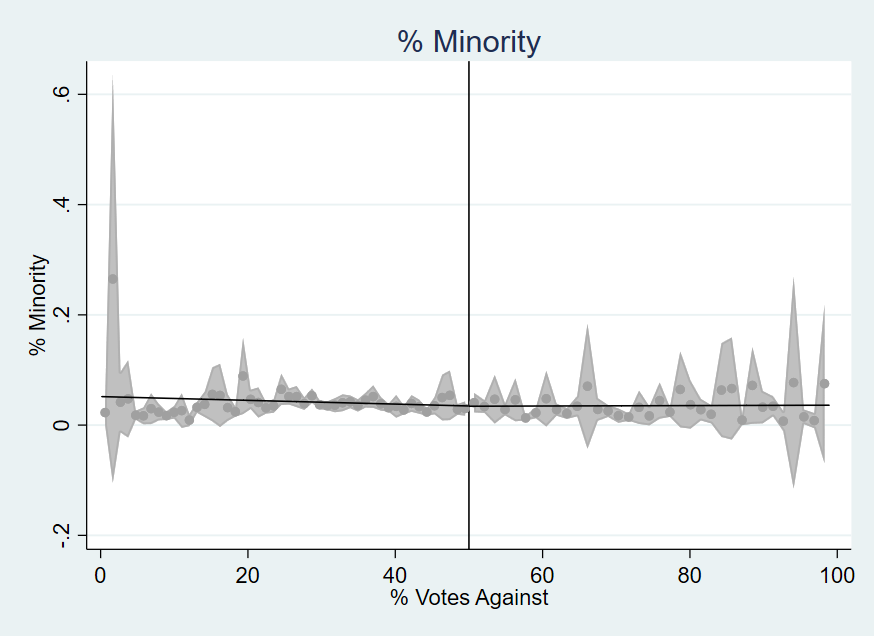
\includegraphics[width=\textwidth,keepaspectratio]{images/cov_smoothness_pctmin.png}
        \caption*{Pct Minority}
        \label{fig:pctmin_sm}
    \end{minipage}
    
    \caption{Covariate Discontinuity Plots - Part 2}
    \label{fig:rd_cov_smoothness_2}
\end{figure}


\clearpage


\section{Additional Information} \label{sec:appxc}

% \subsection{A Case Study of Roads in Waynesville OH: Serial Cutter of Road Maintenance Tax Levies}
\subsection{More Details on Predicting Road Quality} \label{sec:appxc1}

Coming very soon.

\subsection{Road tax levies vs. Other types of levies}

\begin{table}[ht!]
    \centering
    \caption{Correlation of Road Tax Levy Referenda Results with Other Types of Levies}
    \begin{tabular}{lcccccc}
    \toprule
    & Police & Fire & Current Expenses & Recreational & School \\
    \midrule
    Estimate & 0.248 & 0.053 & 0.388*** & 0.015 & -0.024 \\
    & (0.153) & (0.043) & (0.099) & (0.317) & (0.092) \\
    \bottomrule
    \end{tabular}
    \begin{minipage}{\textwidth}
    \footnotesize
    \textit{Notes:} This table presents coefficients from regressions correlating road tax levy referendum outcomes with outcomes for other types of levies (police, fire, current expenses, recreational, school). Standard errors are reported in parentheses. The coefficient for "Current Expenses" is statistically significant at the 1\% level (***). All regression control for year and neighborhood fixed effects, as well as neighborhood characteristics. The school levy analysis is conducted at the county level, while all other analyses are at the county subdivisions level. Statistical significance levels are indicated as follows: *** $p<0.01$, ** $p<0.05$, * $p<0.1$.
    \end{minipage}
\end{table}

% \begin{figure}[ht]
%     \centering
%     \begin{minipage}[b]{0.48\textwidth}
%         \centering
%         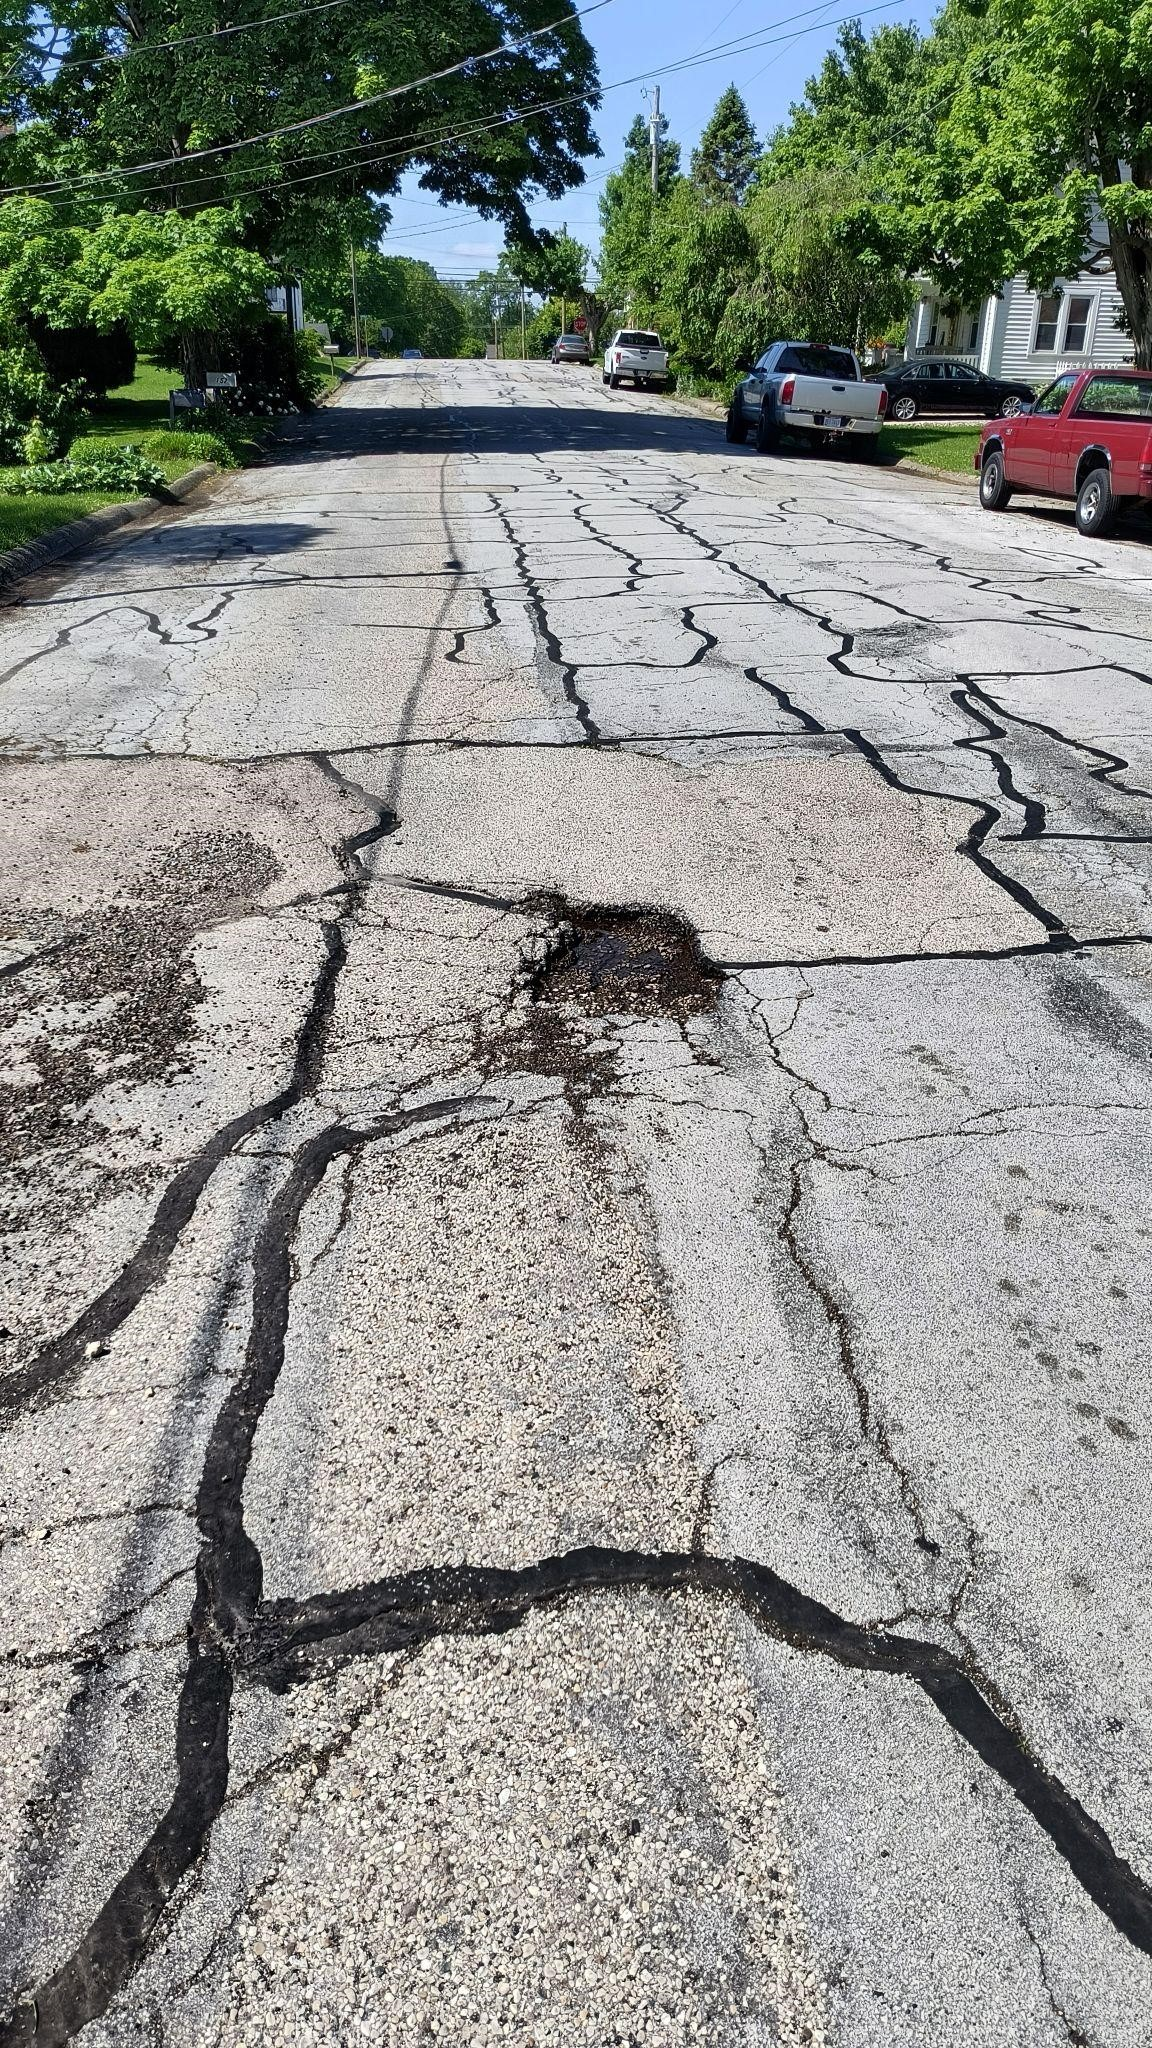
\includegraphics[width=0.75\textwidth,keepaspectratio]{images/waynesville_oh_1.png}
%         \caption*{Waynesville Road Image 1}
%         \label{fig:w_oh_1}
%     \end{minipage}
%     \hfill
%     \begin{minipage}[b]{0.48\textwidth}
%         \centering
%         \includegraphics[width=0.75\textwidth,keepaspectratio]{images/waynesville_oh_2.png}
%         \caption*{Waynesville Road Image 2}
%         \label{fig:w_oh_2}
%     \end{minipage}

%     \vspace{1em}

%     \begin{minipage}[b]{0.48\textwidth}
%         \centering
%         \includegraphics[width=0.75\textwidth,keepaspectratio]{images/waynesville_oh_3.png}
%         \caption*{Waynesville Road Image 3}
%         \label{fig:w_oh_3}
%     \end{minipage}

%     \caption{Roads in Waynesville: Case Study}
%     \label{fig:rd_waynesville}
% \end{figure}

% \section{More Details on Predicting Road Quality} \label{sec:appxd}




\clearpage

% \onehalfspacing

% \section*{Tables} \label{sec:tab}
% \addcontentsline{toc}{section}{Tables}


% \section*{Figures} \label{sec:fig}
% \addcontentsline{toc}{section}{Figures}

%\begin{figure}[hp]
%  \centering
%  \includegraphics[width=.6\textwidth]{../fig/placeholder.pdf}
%  \caption{Placeholder}
%  \label{fig:placeholder}
%\end{figure}




\clearpage

% \section*{Appendix A. Placeholder} \label{sec:appendixa}
% \addcontentsline{toc}{section}{Appendix A}



\end{document}